\begin{savequote}[75mm]
There will come a time when it isn't 'They're spying on me through my phone' anymore. Eventually, it will be 'My phone is spying on me'.
\qauthor{Philip K. Dick}
\end{savequote}

\chapter{Web tracking: how advertising networks collect users' browsing patterns}

\newthought{In the early age of the Internet users enjoyed a large level of anonymity.} At the time web pages were just hypertext documents; almost no personalisation of the user experience was offered. The Web today has evolved as a world wide distributed system following specific architectural paradigms. On the web now, an enormous quantity of user generated data is shared and consumed by a network of applications and services, reasoning upon users expressed preferences and their social and physical connections. Advertising networks follow users' browsing habits while they surf the web, continuously collecting their traces and surfing patterns, since advertising sustains the business model of many websites and applications. Efficient and successful advertising relies on predicting users' actions and tastes to suggest a range of products to buy. Both service providers and advertisers try to track users' behaviour across their product network. For application providers this means tracking users' actions within their platform. For third-party services \emph{following} users, means being able to track them across different websites and applications. It is well known how, while surfing the Web, users leave traces regarding their identity in the form of activity patterns and unstructured data. These data constitute what is called the user's on-line footprint. We analyse how advertising networks build and collect users footprints and how the suggested advertising reacts to changes in the user behaviour.

\section{Background}

Websites use \emph{personalisation services} to provide a tailored experience to their visitors. In order to make their product more personal to the single users they need to keep profiles of their users, collect their in page reading activities and eventually their preferences. This data is then shared to third-party services, accessed and analysed without users? direct consent. Furthermore, records of users? activities are used for different purposes, most unknown to the end user, such as marketing or to provide analytics services back to the original website or application.
Among the data analysed by websites are also included user preferences and social connections. These can be obtained by tracking users across different applications and sites through cookies or open web sessions. Even if the user does not accept cookies or is not logged into a service account, such as their Google, Twitter or Facebook accounts, the web page and third-party services can still try to profile them by using third-party HTTP requests, among other techniques. Within the HTTP request various selectors can be included to communicate user preferences or particular features, in the form of URL variables. Features that might be used by advertising networks and malicious trackers include personalised language or fonts settings, browser extensions, in page keywords, battery charge and status, and so on. These features are then used to identify individual users by restricting the pool of possible candidates among all the visitors in a certain time frame, location, profile of interests. Unique users can then be distinguished across multiple devices or sessions.

In this chapter, have observed how users are tracked across the Web and how the displayed advertising is tailored even after they have visited a few websites with a certain interest bias. In previous work~\cite{puglisi2016web}~\cite{puglisi2015you} we analysed how third-party advertising services are able to profile users on a short series of websites visited and how these are able to \emph{follow} users while they surf the web.
In our study we analyse how the user profile detected by advertising services can be used to estimate the user privacy risk on a certain network. We analyse how advertising networks identify a user and start tracking them, by considering keywords contained in the web-page and understanding the underlying network structure of tracked domains. We measure the distance between the observed user profile and the actual user profile, by categorising the set of keywords contained in web pages and by capturing third-party HTTP requests. We introduce a set of metrics to express this distance between the two profiles.

It is important to note that we have considered the case for which users are not registering, neither connecting any external account, as it could be the case with services like: Facebook, Google+, Twitter, and so on. In such scenario we have measured how these networks still attempt to track the user by sending user information through HTTP requests to their services.

We present a model of the user profile that is able to capture how each website and tracking network categorise their activities in terms of interests and interactions.

Therefore, we analyse how much information is sent by each page visited to third-party services by measuring the partial user profile and the actual user profile. The partial user profile is what the website and third-party services know about the user. The actual user profile is instead the full profile measured at the end of the series of page visited.

We then, introduce a set of metrics to express the relationship between the partial and the actual user profile.

Hence, we profile third-party HTTP calls sent by Facebook tracking services and compare this to the the user actual profile.

Finally, we model user on-line footprints as a graph of the actions generated by each user and analyse the resulting graph structure, identifying known malicious trackers.

\section{Modelling the user profile}
\label{sec:mod-profile}
Each time the user visits a new page, we aggregate the page keywords and build what we consider the user's profile of interests (Figure ~\ref{abs-profile}). We consider a tractable model of the user profile as a probability mass function (PMF), as proposed in~\cite{Parra12DKE,Parra12TKDE}, to express how each keyword contributes to expose how many times the user has indirectly expressed a preference toward a specific category. We consider that the user expresses a preference when they visit a webpage categorised with certain keywords. This model follows the intuitive assumption that a particular category is weighted according to the number of times this has been counted in the user profile.

We define the profile of a user as the PMF $p = (p_1,\ldots, p_L)$, conceptually a histogram of relative frequencies of tags across the set of tag categories $\mathcal{T}$. This means that we group tags around interests using top level categories as defined by the Open Directory Project (DMOZ)~\cite{a22}.
The user profile is calculated at the end of the series of website visited by the user. Similarly we define the partial user profile at moment as this is known to the advertising network as  $\hat{p} = (\hat{p}_1,\ldots, \hat{p}_L)$.

Note that, for the case when an advertising network is present on each and every page, $\hat{p} = p$ at the end of the series of sites visited. This means that the network was able to record each page visited by the user. This could easily be the page of advertising networks like Google that through different third-party services are ubiquitously present across the web.

We also define the profile of an ad, or third-party http request as the PMF $q =(q_1,\ldots, q_L)$, where $q_l$ is the percentage of tags belonging to the category $l$ which have been assigned to this specific advertising item. You can think of the ad profile as the PMF of the tag contained in every http request sent from the visited page to the advertising network (Listings: ~\ref{amazon}, ~\ref{krxd}, ~\ref{facebook}). This profile notes which tags the tracking network is using to identify the user and display some advertising content. Note that the ads profile, is calculated independently for each advertising network.

Both user and ads profiles can then be seen as normalised histograms of tags across categories of interest. Our profile model is in this extent equivalent to the tag clouds that numerous collaborative tagging services use to visualise which tags are being posted, collaboratively or individually by each user. A tag cloud, similarly to a histogram, is a visual representation in which tags are weighted according to their relevance.

In view of the assumptions described in the previous section, our privacy attacker boils down to an entity that aims to profile users by representing their interests in the form of normalised histograms, on the basis of a given categorisation.

We consider the third-party advertising network to operate like a recommendation system that suggest products or services that might be of interest for the user, based on their preferences. A recommendation system can be described as an information filtering system that seeks to predict if the user is interested or not in a particular resource. We assume that the ad server suggests advertising based on a measure of \emph{similarity} between what the user \emph{does} and what the network \emph{knows}. Furthermore, we consider tracking service to work in a feedback loop (Figure: ~\ref{fig:advertising-loop}). When a user surfs the web each tracker on the visited pages communicates with the advertising service, sending a number of parameters through HTTP requests. These contain the user preferences and browsing history which will be taken into consideration when ads are returned to display on the page.

It is important to note that while it is safe to consider an advertising network as a recommendation system, we should also consider that a number of processes and interactions between the advertising networks, the website, and the ultimate advertiser, can influence the actual recommendation that is displayed to the user. Tracking services can in fact follow different strategies to recommend products to users. Some services display in page advertising where a bidding mechanism allow advertisers to compete for categories and spaces, other services might decide to target only specific categories, others might instead decide to target the visited page only.

\begin{figure}
\centerline{\epsfxsize=350pt\epsfbox{figures/advertising-loop.png}}
\caption[Advertising services feedback loop]{Advertising services work in a feedback loop. The image illustrate how while a user surf a number of web pages, the service record their profile and adapts the returned advertising.}
\label{fig:advertising-loop}
\end{figure}

We measure the user profile, as previously described, as a histogram of their recorded preferences, and the advertising profile as a histogram of the ads that the user has received. We have considered a set of metric to measure how the advertising network is tracking the user profile, and how a page sends information to a tracking service by transmitting a partial user profile.

In previous works\cite{puglisi2016web}~\cite{puglisi2015you} we used the \emph{1-norm}, \emph{2-norm} as measures of how the advertising profile, or the partial user profile, approximates the user profile. Please recall that the partial user profile is calculated by a given advertising network at a given moment on a series of pages visited.

We now introduce the normalised \emph{$\alpha$-norm} as the generalised variation \mathcal{GV} between two probability distributions, the partial and the genuine user profiles. Furthermore, we will introduce the \emph{KL-divergence} as a measure of how the partial profile approaches the genuine user profile. Please note that while we are defining our metrics between the partial user profile and the genuine user profile, the same assumptions holds, without loss of generality, if we compare the user's and the advertising profiles.

\subsubsection{Norm and generalised variation}

We define the $\alpha-norm$ between the partial profile as observed by an advertising platform and the genuine user profile as:

$$ \| p - \hat{p} \|_\alpha = \sqrt[\alpha]{\sum_l{ {| p_l - \hat{p}_l |}^\alpha }} \quad  \text{with} \quad  \alpha \in [0, \infty] $$

The case for $\alpha = \infty$ is defined in the limit:

$$\lim_{\alpha\to\infty} \| p - \hat{p} \|_\alpha = \lim_{\alpha\to\infty} \sqrt[\alpha]{\sum_l{ {| p_l - \hat{p}_l |}^\alpha }} \approx \max_l { | p_l - \hat{p}_l | } $$

The $\alpha-norm$ is a distance in $\mathbb{R}^L$ with the following properties:

\begin{itemize}
 \item Absolute homogeneity.
 \item Positive definite: $ \| p - \hat{p} \|_\alpha = 0 \Leftrightarrow p = \hat{p} $ and $ \| p - \hat{p} \|_\alpha = \sqrt[\alpha]{2}$ $\Leftrightarrow$  $p$ and $\hat{p}$ are orthogonal deltas.
 \item Triangle equality.
\end{itemize}

For $\alpha = 1$ we define the \emph{1-norm} between the partial and the genuine user profiles as:

$$ \| p - \hat{p} \|_1 = \sum_l{ | p_{l} - \hat{p}_{l} | }  $$

The \emph{1-norm} represent the average discrepancy between the two profiles. For $\alpha = 2$ we define the \emph{2-norm} as:

$$ \| p - \hat{p} \|_2 = \sqrt{\sum_l{ {| {p_{l} - \hat{p}_{l}} |}^2 }} $$

The \emph{2-norm} represents the Euclidean distance between the two distributions. When considering the \emph{2-norm} it is possible to highlight larger discrepancies on the set of categories analysed. An interesting property is that \emph{norms} are also nested. Hence:

$$ \| p - \hat{p} \|_\infty \leqslant \| p - \hat{p} \|_2 \leqslant \| p - \hat{p} \|_1 $$

We hence define the generalised variation $\text{GV}(p, \hat{p})$, based on $\alpha$-norm as:

$$ \text{GV}(p, \hat{p})_\alpha = \frac {1} {\sqrt[\alpha]{2}}  {\| p - \hat{p} \|}_\alpha =  \frac {1} {\sqrt[\alpha]{2}} \sqrt[\alpha]{{ \sum_l{ ( p_{l} - \hat{p}_{l})^\alpha } }} ,\quad  \alpha \in [1,\infty]$$

The coefficient $\frac {1} {\sqrt[\alpha]{2}}$ normalises the range of values of the \emph{$\alpha-norm$} in $[0, 1]$. Therefore, $\text{GV}(p, \hat{p})$ is a norm, is positive definite, absolutely homogeneous and satisfies the triangle inequality:

\begin{itemize}
 \item $\text{GV}(p, \hat{p}) \geq 0 $ with equality if and only if $p = \hat{p}$
 \item $\text{GV}(p, \hat{p}) \leq 1$ with equality if and only if $p$ and $\hat{p}$ are orthogonal canonical vectors (discrete deltas).
\end{itemize}

Note that for $\alpha = 1$ the generalised variation $\text{GV}(p, \hat{p})$ is equal to the total variation $\text{TV}(p, \hat{p}) $:

$$ \text{TV}(p, \hat{p})= \frac {1} {2}  \| p - \hat{p} \|_1 =  \frac {1} {2} \sum_l{ | p_{l} - \hat{p}_{l} | } $$

For $\alpha = 2$ we have the normalised \emph{2-norm}:

$$ \text{GV}_2 = \frac {1} {\sqrt{2}}  {\| p - \hat{p} \|}_2 =  \frac {1} {\sqrt{2}} \sqrt{{ \sum_l{ | p_{l} - \hat{p}_{l}|^2 } }} $$

Finally, the case for $\alpha = \infty$, $\lim_{\alpha\to\infty} \text{GV}(p, \hat{p})_\alpha = \| p - \hat{p} \|_\infty $ between $p$ and $\hat{p}$. The reason is that for $\alpha \gg 1$ the greatest difference dominates in the sum $\sum_l{ {| p_l - \hat{p}_l |}^\alpha }$. Therefore $\lim_{\alpha\to\infty} \| p - \hat{p} \|_\alpha \approx \max_l { | p_l - \hat{p}_l | } $.

One might interpret these norms as $\alpha = 1$ been an average-case metric, $\alpha=\infty$ being a worst-case scenario, and $\alpha=2$ a robust middle ground.

\subsubsection{KL-Divergence}

Now we propose and justify an information-theoretic quantity as a measure of how the partial profile approaches the genuine user profile: the \emph{KL-divergence}. Suppose that we might interpret the profile $\hat{p}$ observed by a third-party tracking service, as a sequence of $L$ independent, identically distributed, drawings of a user's genuine profile of interest $p$. Then in accordance with the rationale proposed in ~\cite{parra2014measuring}~\cite{rebollo2011information}, we may argue that the probability $p(\hat{p})$, of a given observed profile is related to the KL-divergence between the empirical observation $\hat{p}$ and the ideal one $p$, as follows:

$$ - \frac {1}{L} \log{p(\hat{p})} \xrightarrow[L \to \infty]{} \textnormal{D}(\hat{p} \| p) $$

Informally this means $p(\hat{p}) \approx 2^{-\textnormal{L D}(\hat{p} \| p) } $. Note that small divergences will lead to likely outcomes, whereas large divergence associate with rare events.

Note also that $\hat{p}$ is absolutely continuous with respect to $p$: $p_l = 0 \Rightarrow \hat{p}_l = 0$. Also $\hat{p} \ll p \iff  \textnormal{D}(\hat{p} \| p) < \infty$.

\section{Modelling the user's on-line footprint}
We model the user's activity as series of events belonging to a certain identity. Each event is a document containing different information. An event correspond to an action generated by the user or one of their devices. When a user visits a website or creates a post on a blog, an event is created. We can think of an event as a hypermedia document i.e. an object possibly containing graphics, audio, video, plain text and hyperlinks. We call the hyperlinks selectors and we use these to build the connections between the user's different identities or events. Each identity can be a profile or account that the user has created onto a service or platform, or just a collection of events, revealing something about the user. With account we mean an application account or a social network account, such as their LinkedIn or Facebook unique IDs. When the user visit a web page, or uses a web or mobile application, a series of events is generated and associated with the account. Some of these events are created by direct user's actions, others are created by code triggered indirectly by the user.

While the user visits a webpage and reads its content a series of snippets of code and client side scripts are executed and information is transmitted to the page backend or some third-party server. Among the information transferred are a number of user preferences. These can be their geographical location, battery level of their current used device, browser preferences, or just their browsing history captured up to that point. Some or all of the meta and in page keywords used to describe the page are also transferred. We build the user profile by collecting the meta keywords expressed in web pages. We consider this a subset of the possible set of preferences that third-party advertising networks might be interested in collecting.

\subsection{Proposing a model of third-party requests on web pages}

When a user visits a web page, the browser sends an http request to the server to request a representation of the resource described through the url. The server provides the resource representation in the form of a html document and the browser parses it. The html document contains a number of links to other resources, such as JavaScript code, videos, audios or images (Figure: ~\ref{third-party}). Some of these can be stored on the same domain as the requested page, some may be requested to third-party services. Such is the case of services like Google Analytics, share buttons from different social networks, or advertising banners. Together with the http request, a number of parameters are included. These contains keywords, users? preferences, information regarding the user device and session, in page information sent to the third-party service from the website or application.

\setcounter{figure}{1}
\begin{figure}
\centerline{\epsfxsize=350pt\epsfbox{figures/tracker-request.png}}
\caption{Trackers on web pages make third-party http requests to advertising services. These return ads content tailored to the user web history or expressed preferences.}
\label{third-party}
\end{figure}

When a third-party request is performed by the visited page, we store the parameters passed and if the call belongs to a known tracking network we categorise the corresponding keywords. Also when a request is made, we store a direct link between the page and a tracking domain, such as google.com. This results in a graph model of tracking networks and how these are connected to pages (Figure: ~\ref{graph-map}). The graph model allows us to understand the underling network structure of tracking networks and how these are pervasively following users across their visits. In fact, every time we discover which tracking services are active on a certain website, we can create an indirect link between the user and the tracker.

\setcounter{figure}{2}
\begin{figure}
\centerline{\epsfxsize=350pt\epsfbox{figures/graph-map.png}}
\caption{The graph shows how known trackers are connected to visited pages and therefore how these are able to follow users across different websites.}
\label{graph-map}
\end{figure}

\subsection{Network structure metrics}

We said that advertising networks or privacy attackers need to be able to \emph{follow} the user across as many websites as possible in order to profile their interests. This naturally translates onto a graph model where each page is directly connected to its active trackers (Figure: ~\ref{graph-map}).
We therefore considered a set of metrics that can uncover the underlying network structure of tracking service. The first of the metrics considered is the average degree of the neighbourhood. The average degree of the neighbourhood of each node is a good indication of how many pages are connected to a certain advertising service or tracking domain.

The average degree of the neighbourhood of a node $i$ is calculated as:

$$ \langle k_{nn,i} \rangle= \frac{1}{| N(i) |} \sum_{j \in N(i) } {k_j} $$

Where $N(i)$ are the neighbours of node $i$ and $k_j$ is the degree of node $j$ which belongs to $N(i)$.

If a certain tracker domain is connected to the majority of the page visited by a certain user, this means that they have been able to collect the user's preferences and reading activities across a number of websites. The more a tracker domain is connected, the more the user might consider this a \emph{risk} for their privacy. We used the average degree of the neighbourhood of a tracker to rank tracker domains.

To describe the resulting network structure we also calculated the average scalar assortativity coefficient~\cite{newman2002assortative} defined as:

$$ r = \frac{\sum_{xy} xy(e_{xy} - a_x b_y)}{\sigma_a\sigma_b} $$

Where $a_x=\sum_ye_{xy}$ and $b_y=\sum_xe_{xy}$, and $e_{xy}$ is the fraction of edges from a vertex of type x to a vertex of type y.

We also generated a partition of SBM and nested SBM of the resulting graph employing an agglomerative multilevel Markov chain Monte Carlo (MCMC) algorithm as described in~\cite{peixoto2014efficient}~\cite{peixoto2013parsimonious}\cite{peixoto2012entropy}. The idea behind using SBM to describe the network structure of identified trackers is to be able to identify similar trackers and to understand if trackers belonging to the same domain or that exhibit similar behaviour can be grouped based on network properties.

\setcounter{figure}{3}
\begin{figure}
\centerline{\epsfxsize=350pt\epsfbox{figures/absolute-population-profile.eps}}
\caption{Here we show an example of user profile expressed in absolute terms by counting the number of keywords in each category for a browsing session. We model user and advertising profiles as histograms of tags keywords a set of predefined categories of interest.}
\label{abs-profile}
\end{figure}

\begin{table}[htbp]
\centering
\caption{\label{tableDatasetStats} Statistics regarding collected users data}
\def\arraystretch{2.5}
\begin{tabular}{| l | r | l | r | }
\hline
\multicolumn{4}{|c|}{Statistics about collected data}            \\[2.5mm] \hline
Categories               & 16    & Users                   & 50   \\[2.5mm] \hline
Pages per users    & 100 & Total pages      & 5000 \\[2.5mm] \hline
\end{tabular}
\end{table}

We profiled 50 users and each user visited a series of 100 pages. In total we analysed 5000 different pages (Table: ~\ref{tableDatasetStats}). For each user we calculated how each page contributed to the user profile and also how third-party services adapted to the user profile by returning certain information in form of ads. Information that advertising services request from the visited page may vary in length and type (Listings: ~\ref{amazon}, ~\ref{krxd}, ~\ref{facebook}). Some trackers might include only the referrer \emph{url} and some devices information and user triggered parameters (Listings: ~\ref{amazon}, ~\ref{facebook}) while other services might be more lengthily in what is sent from the page (Listing: ~\ref{krxd}). Some of the information sent through third-party request cannot be categorised, since they include hashed users? ids and internal keywords and code belonging to the tracking service. Other information, like the keywords retrieved from the page (Listing: ~\ref{krxd}) can be categorised into category of interest that we assume the tracking service uses to profile the user through their interests.

It is interesting to not how among the parameters sent to the third-party tracking services are not included just in page keywords regarding the topic of the page, but also specific browser information. Some of the device's preferences are included in the http headers, like the user-agent identifying the browser and the Operative System. Other information regard how long the page took to load or how soon the content was ready (Listing: ~\ref{krxd}).

\lstset{caption={A third-party request to Amazon Ads Service from the nytimes.com homepage. In this example keywords are sent directly as parameters in the http request.},label=amazon}
\begin{lstlisting}[frame=single, breaklines=true, keepspaces=true, basicstyle=\tiny, escapechar=!]
Host: !\textcolor{red}{aax.amazon-adsystem.com}!
User-Agent: Mozilla/5.0 (Macintosh; Intel Mac OS X 10.11; rv:48.0)
Gecko/20100101 Firefox/48.0
Accept: */*
Accept-Language: en-US,en;q=0.5
Accept-Encoding: gzip, deflate
DNT: 1
Referer: !\textcolor{red}{http://www.nytimes.com/2016/08/29/us/politics/donald-trump-congress-gop-voters.html?hp}!
Params:
	action: click
	pgtype: Homepage
	clickSource: story-heading
	module: first-column-region
	region: !\textcolor{red}{top-news}!
	WT.nav: top-news
	_r: 0
Cookie: ad-id=A8rOwZ2wOUK4gka1zjqyWNo; ad-privacy=0
Connection: keep-alive
\end{lstlisting}

\lstset{caption={A third-party request to krxd.net from a nytimes.com article. This request send different information regarding the article and the browser preferences through http parameters. In addition to the keywords associated with the page, we can see how the request includes information regarding how long it took for the content to be ready \(param: t_content_ready\) as well as how much it took for the browser window to load \(param: t_window_load\).},label=krxd}
\begin{lstlisting}[frame=single, breaklines=true, keepspaces=true, basicstyle=\tiny, escapechar=!]
GET /pixel.gif?
Params:
	source: smarttag
	_kcp_s: nytimes
	_kcp_sc: !\textcolor{red}{us}!
	_kcp_ssc: !\textcolor{red}{politics}!
	_kcp_d: www.nytimes.com
	_kpref_: http://www.nytimes.com/
	_kua_kx_lang: en-us
	_kua_kx_tech_browser_language: en-us
	_kpa_page_type=article
	_kpa_cg: us
	_kpa_scg: politics
	_kpa_pst: !\textcolor{red}{News}!
	_kpa_des: !\textcolor{red}{Presidential Election of 2016}!
	_kpa_per: !\textcolor{red}{Lujan Ben Ray}!
	_kpa_org: !\textcolor{red}{Republican Party}!
	_kpa_author: !\textcolor{red}{Alexander Burns and Jonathan Martin}!
	_kpa_keywords2: !\textcolor{red}{Presidential Election of 2016 Elections House of Representatives Politics Action Committees Elections Senate Republican Party Lujan Ben Ray Issa Darrell Trump Donald}!
	t_content_ready: !\textcolor{red}{1792}!
	t_window_load: !\textcolor{red}{12720}!
	...
Host: !\textcolor{red}{beacon.krxd.net}!
User-Agent: Mozilla/5.0 (Macintosh; Intel Mac OS X 10.11; rv:48.0) Gecko/20100101 Firefox/48.0
Accept: */*
Accept-Language: en-US,en;q=0.5
Accept-Encoding: gzip, deflate
DNT: 1
Referer: http://www.nytimes.com/2016/08/29/us/politics/donald-trump-congress-gop-voters.html?hp&action=click&pgtype=Homepage&clickSource=story-heading&module=first-column-region&region=top-news&WT.nav=top-news&_r=0
Cookie: ServedBy=beacon-a262-dub; _kuid_=DNT
Connection: keep-alive
\end{lstlisting}

\lstset{caption={A third-party request to facebook.com from a indipendent.co.uk article.},label=facebook}
\begin{lstlisting}[frame=single, breaklines=true, keepspaces=true, basicstyle=\tiny, escapechar=!]
Host: !\textcolor{red}{graph.facebook.com}!
User-Agent: Mozilla/5.0 (Macintosh; Intel Mac OS X 10.11; rv:48.0) Gecko/20100101 Firefox/48.0
Accept: */*
Accept-Language: en-US,en;q=0.5
Accept-Encoding: gzip, deflate, br
DNT: 1
Referer: http://www.independent.co.uk/news/uk/politics/europe-could-go-down-the-drain-after-brexit-a7213976.html
Cookie: datr=TbHdVa-yyYq_3UHH_xYR6NGb; fr=0MuKlsg7QM3etJaWt.AWVJMdGky_V9X82TY03Y-wBtGqE.BV3bFx.XF.FfD.0.0.BXw9oU.AWVWPpAJ; lu=TggRyE6qvvdCystV9I2G-b0w; _ga=GA1.2.1182524233.1441193978; sb=i14HV4ufa1WguCxPntCQagP0; c_user=100007394807876; xs=192%3AnWrYMasjLyLusw%3A2%3A1365011662%3A5189; csm=2; s=Aa4hJAWUyE0HSY_M.BXj1Ln; pl=n; p=-2; act=1472453154239%2F0; presence=EDvF3EtimeF1472453144EuserFA21B07394807876A2EstateFDutF1472453144216Et2F_5b_5d
    Elm2FnullEuct2F1472410836BEtrFA2
    loadA2EtwF240195646EatF1472453143045CEchFDp_5f1B07394807876F2CC
Connection: keep-alive
\end{lstlisting}

Once we were able to collect and profile readable keywords from http requests, we wanted to know how each page contribute to \emph{how much tracking services know} about our genuine user profile by observing a series of web pages visited.
For each users we calculated the \emph{TV}, the \emph{$GV_2$}, the \emph{$\infty$-norm} and the \emph{KL-divergence} between the partial and the genuine user profile (Figure: ~\ref{average-pop-profiles}).
The metrics were calculated for 80 visited, while the genuine user profile was calculated over a series of 100 visits. Therefore, in our scenario, if a tracker is present in each visited page they would \emph{know}, in the worst case scenario 80\% of the visited pages.
Note that the \emph{TV} gives a measure of the average discrepancy between the probability distributions, while the \emph{$\infty$-norm} gives the worst case scenario. From our results we see that the worst case scenario and the average one behave similarly.

We have then analysed the case of a tracker that is not present in each of the visited pages. We considered the facebook third-party requests to their services for this experiment. For each user we calculated the \emph{TV}, the \emph{$GV_2$}, the \emph{$\infty$-norm} and the \emph{KL-divergence} between the partial and the genuine user profile (Figure: ~\ref{average-facebook-pages-tracker}) for pages where the tracker is present.

Finally we profiled keywords in third-party http requests to Facebook. We wanted to know what information were sent to Facebook for each page visited where the tracker was present. This is important to understand what trackers are able to capture about users preferences if they are not able to \emph{follow} the user across all the pages visited. We assumed that if a tracker is not present on a page, they have no knowledge the user visited it, therefore the partial profile as it is known to the tracker is not modified.

Note also that although none of the users considered in our experiment where logged into Facebook, web pages consistently send data to their third-party tracking services. This means that users are profiled by Facebook even if these are not logged in their platform, and individuals that have decided to opt out of Facebook continue to be targeted and known to their services. This is evident by the request shown on listings~\ref{facebook}. A number of browser and device specific information is collected by the http call although the user isn't connected to Facebook. For each users we calculated the \emph{TV}, the \emph{$GV_2$}, the \emph{$\infty$-norm} and the \emph{KL-divergence} between the advertising profile $q$ and the genuine user profile $p$ (Figure: ~\ref{average-facebook-tags-tracker}) for pages where the tracker is present. We considered a shorter series of pages (15 pages) following the intuition that advertising networks might try to form a profile of the user instantly given a small number of visits to similar pages. This was consistent with previous results obtained~\cite{puglisi2015you}.

We have also analysed network structure among the discovered trackers. By using our footprint model we also considered how tracker domains are linked to pages. In this case we calculated the average degree of the neighbourhood of each node, for nodes corresponding to advertising services. Our results show how it is possible to identify known tracker domains by measuring the average degree of the neighbourhood (Table: ~\ref{tabletrackers}).

Considering the average degree of the neighbourhood of each node, we can also find out about some interesting properties of the network. We started considering the \emph{in-degree distribution} of the network (Figure: ~\ref{deg-dist}). The degree distribution $P(k)$ of a network is defined as the fraction of nodes in the network with degree $k$. It is particularly interesting to note that the network \emph{in-degree distribution} approximately follow a power law.

Another interesting property to consider is \emph{assortativity}. Assortativity considers the conditional probability that a node of degree k is connected to a node with degree k'. If the probability function is increasing, the network is said to be assortative, showing that nodes of high degree are more likely to connect to nodes of high degree. If the function is decreasing the network is dissortative, meaning nodes of high degree are more likely to connect to nodes of lower degree. We found that the scalar assortative coefficient for the resulting graph is of -0.19 a value that is often found for internet systems ~\cite{noldus2015assortativity}.

\begin{table}[h!]
\centering
\begin{tabular}{ || c | c || }
\hline
Tracker domain & avg $k_{nn,i}$ \\
\hline
\hline
tacoda.at.atwola.com & 180.0 \\
bcp.crwdcntrl.net & 180.0 \\
match.prod.bidr.io & 180.0 \\
glitter.services.disqus.com & 180.0 \\
ad.afy11.net & 180.0 \\
idsync.rlcdn.com &180.0 \\
mpp.vindicosuite.com & 180.0 \\
aka-cdn-ns.adtechus.com & 180.0 \\
clients6.google.com & 180.0 \\
i.simpli.fi & 180.0 \\
ads.p161.net' & 180.0 \\
dis.criteo.com & 180.0 \\
ads.stickyadstv.com & 180.0 \\
cms.quantserve.com & 180.0 \\
ads.yahoo.com & 129.0 \\
graph.facebook.com & 118.0 \\
ib.adnxs.com & 110.0 \\
rs.gwallet.com & 108.0 \\
bid.g.doubleclick.net & 98.333\\
googleads4.g.doubleclick.net & 98.333\\
\hline
\end{tabular}
\\[2.5pt]
\caption{\label{tabletrackers} The table shows the top 20 identified tracker domains based on the average degree of the neighbourhood.}
\end{table}

We also generated a partition of SBM and nested SBM of the resulting graph (Figures: ~\ref{blockmodel} and ~\ref{blockstate}). Here we identified how the resulting network partitions and communities corresponds to know tracker domains. This means tracking service exhibit similar properties across the same domain and its structure can be identified through statistical inference over the graph.

Furthermore we also computed page-rank algorithm among the network and identified most connected tracked domains (Figure: ~\ref{pagerank}). Again we were able to spot known tracker domains.

\setcounter{figure}{4}
\begin{figure}
\centerline{\epsfxsize=350pt\epsfbox{figures/deg-dist.pdf}}
\caption{\label{deg-dist} Degree distribution for the network resulting from the footprint model of users activity. We can see how the degree distribution follows a power law.}
\end{figure}

\setcounter{figure}{5}
\begin{figure}
\centerline{\epsfxsize=350pt\epsfbox{blockmodel.pdf}}
\caption{\label{blockmodel} Block-model decomposition of the network. We can see how we can identify known tracker networks, and how trackers can be grouped into communities that exhibits similar network structure. The blue squares represent the block partition of the network. While the legend is referred to the original nodes, here represented by the shapes on the border.
}
\end{figure}

\setcounter{figure}{6}
\begin{figure}
\centerline{\epsfxsize=350pt\epsfbox{figures/blockstate.pdf}}
\caption{\label{blockstate} Blockstate representation of the network of tracking service resulting from our simulation. Here we highlight connections between known tracker networks and visited page.}
\end{figure}

\setcounter{figure}{7}
\begin{figure}
\centerline{\epsfxsize=350pt\epsfbox{figures/pagerank.pdf}}
\caption{\label{pagerank} Pagerank computed over the tracking network. Known tracker domains that are \emph{more connected} can be seen with a bigger node symbol compared to less connected ones.}
\end{figure}

\begin{figure}{8}
\begin{center}
\subfigure[]{
\resizebox*{7.5cm}{!}{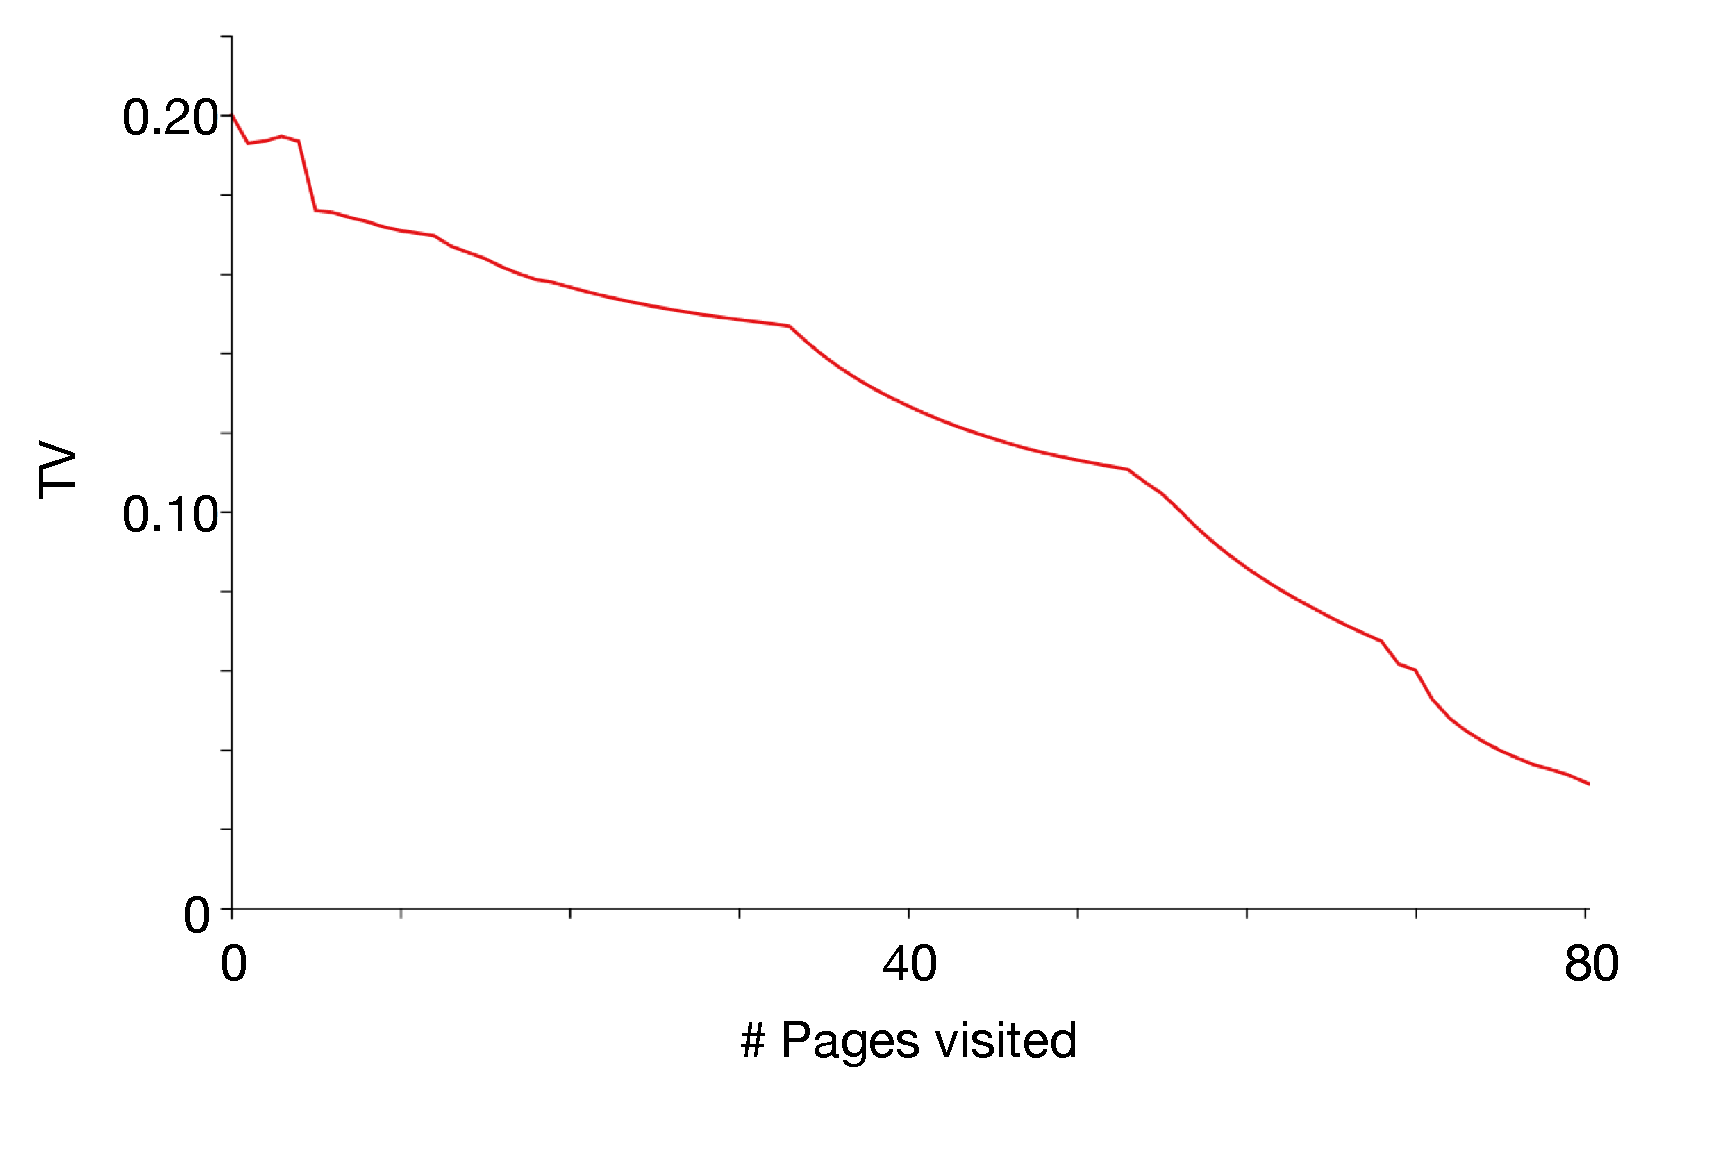
\includegraphics{figures/average_1_norm.eps}}}%
\subfigure[]{
\resizebox*{7.5cm}{!}{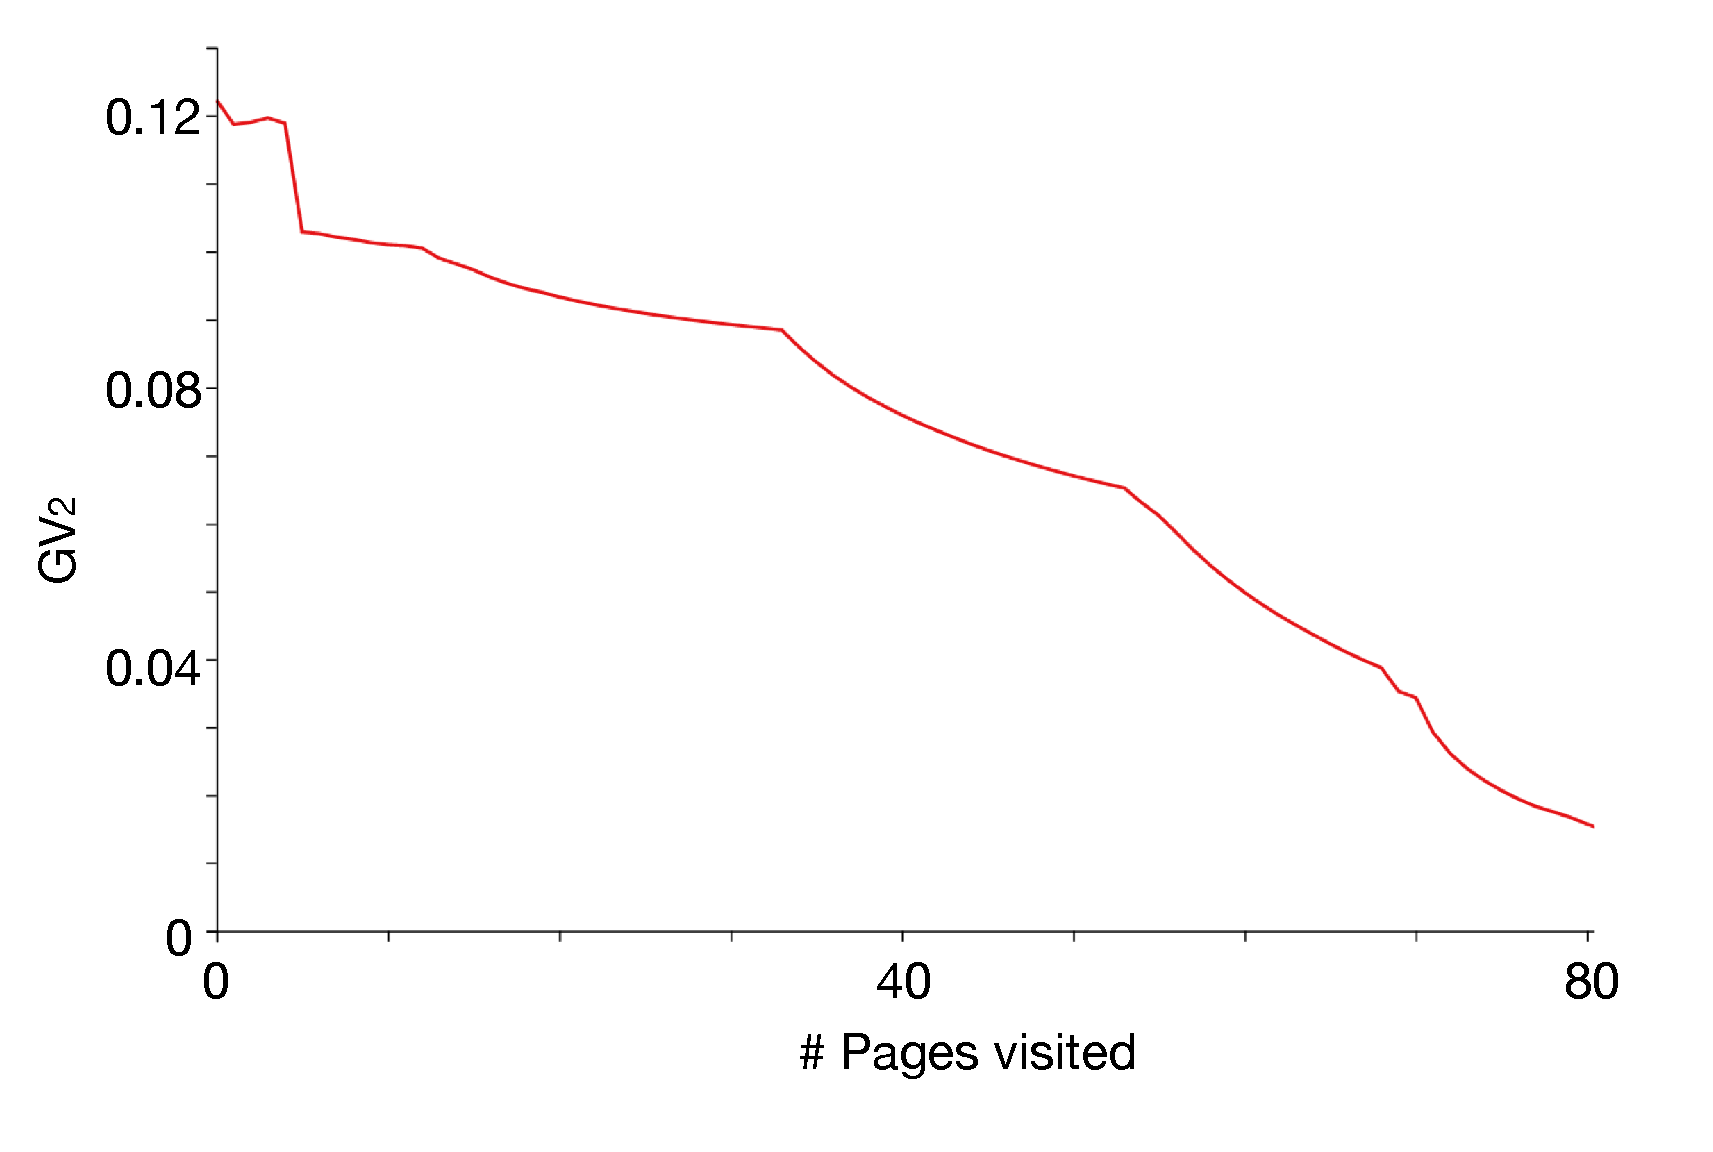
\includegraphics{figures/average_2_norm.eps}}}%


\subfigure[]{
\resizebox*{7.5cm}{!}{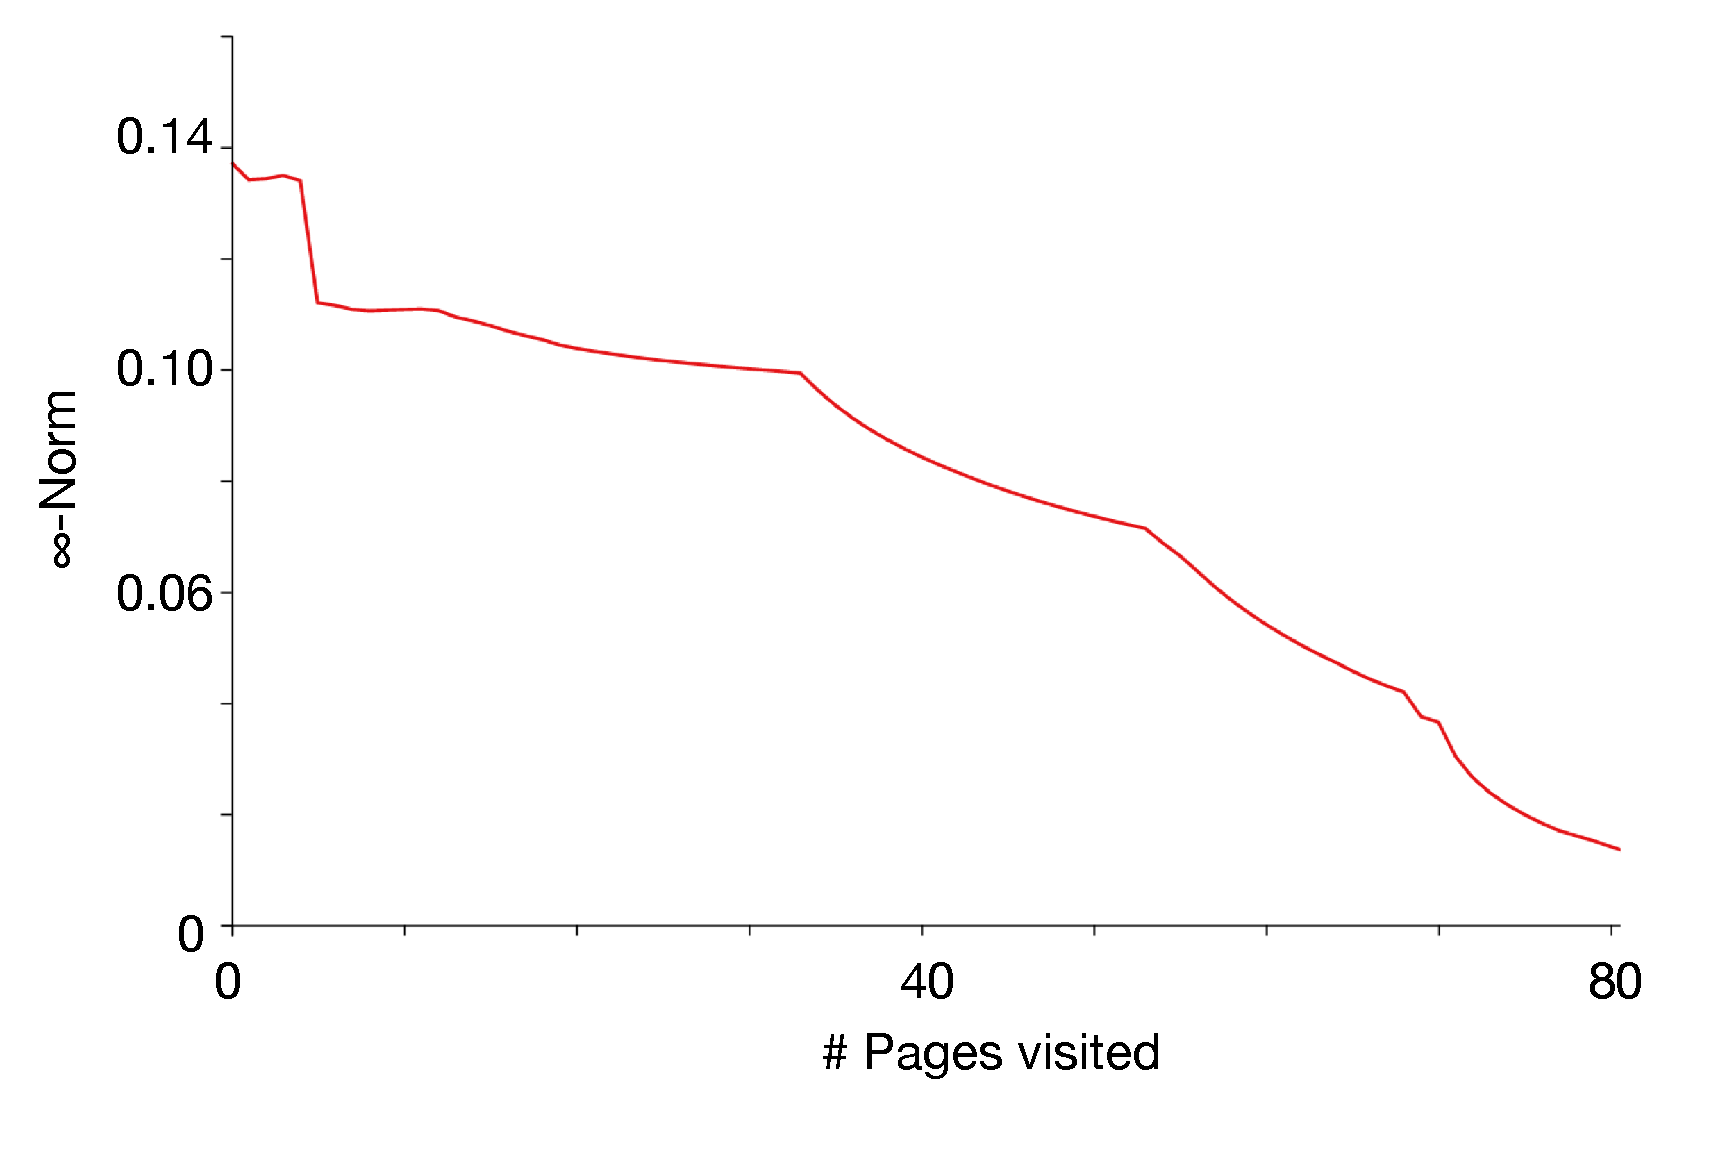
\includegraphics{figures/average_inf_norm.eps}}}%
\subfigure[]{
\resizebox*{7.5cm}{!}{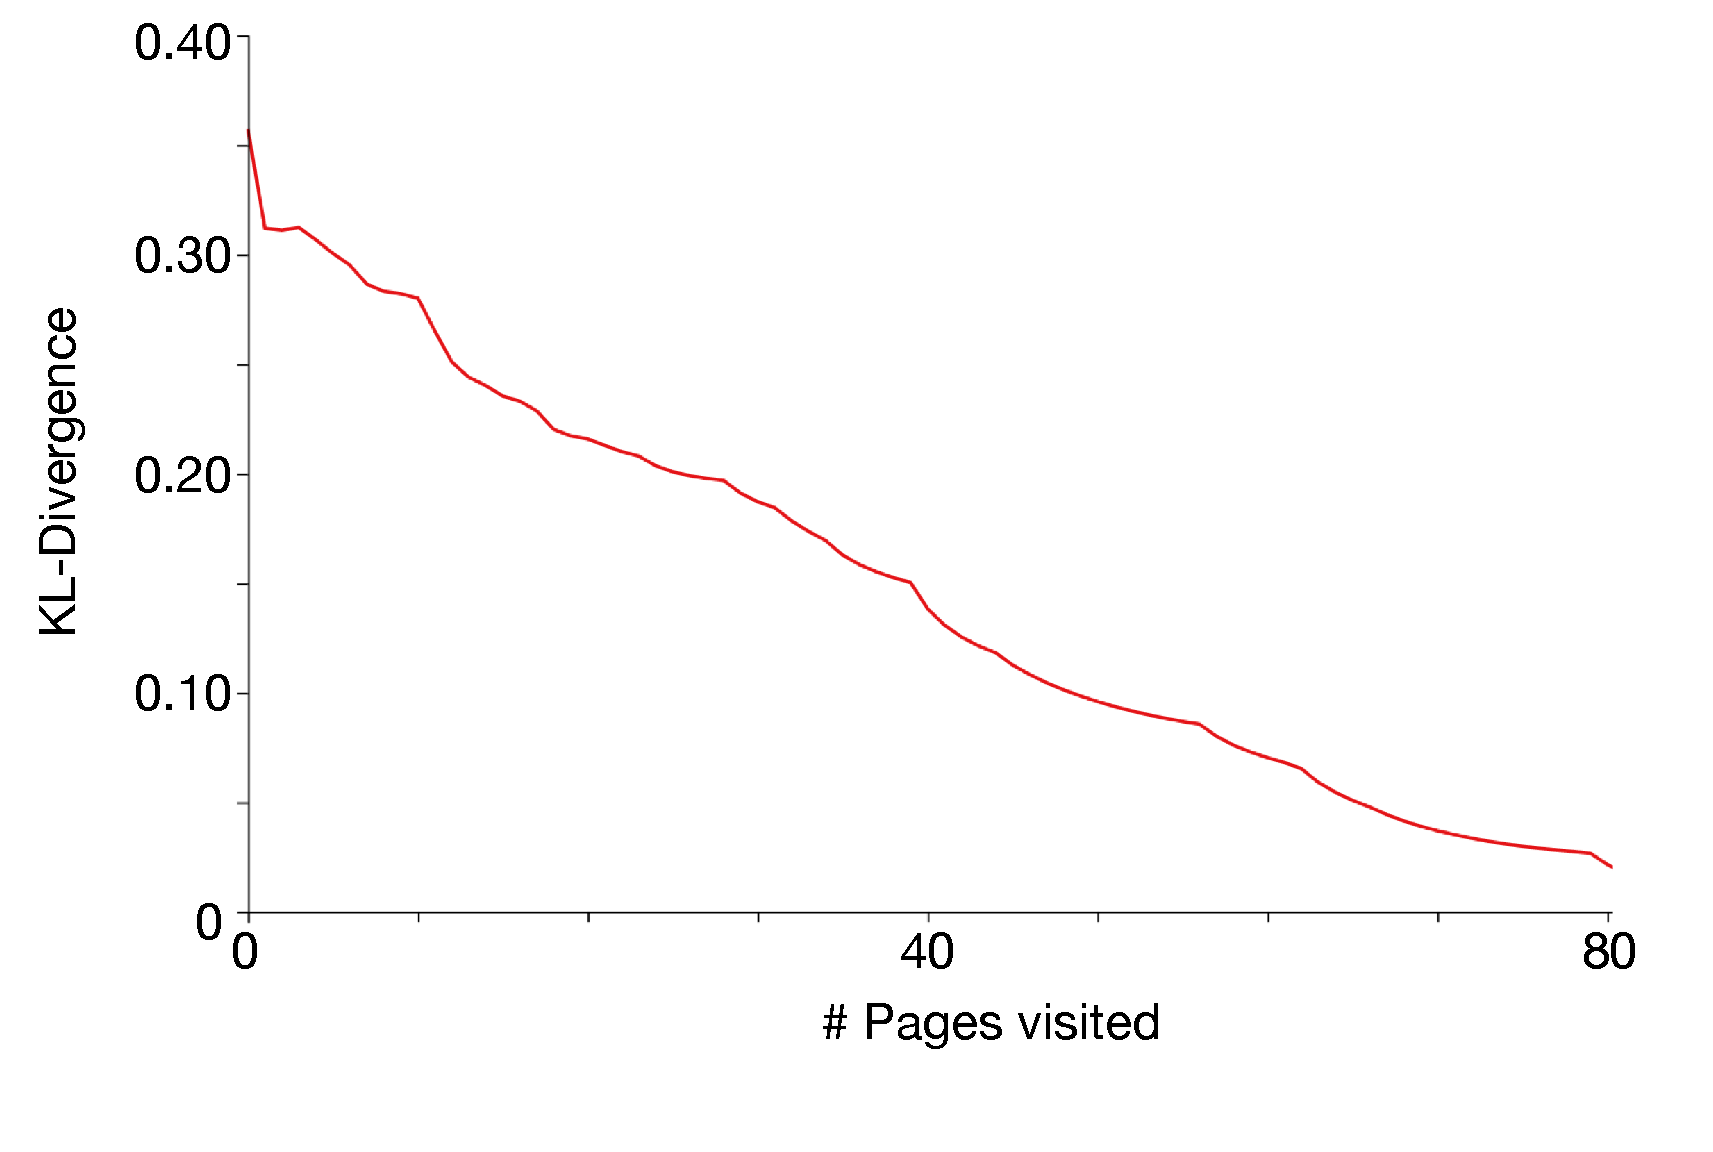
\includegraphics{figures/average_kl.eps}}}%
\caption{\label{average-pop-profiles} The figures show how each page visited contribute to the actual user profile. Please recall that we calculated the user profile at the end of the series of 100 web pages visited and we calculated the metrics for 80 visits, giving a 80\% estimation. %
We therefore computed the \emph{TV}(a), the \emph{$GV_2$}(b), the \emph{$\infty$-norm}(c) and the \emph{KL-divergence}(d) for all pages and averaged among all users.}%
\end{center}
\end{figure}

\begin{figure}{9}
\begin{center}
\subfigure[]{
\resizebox*{7cm}{!}{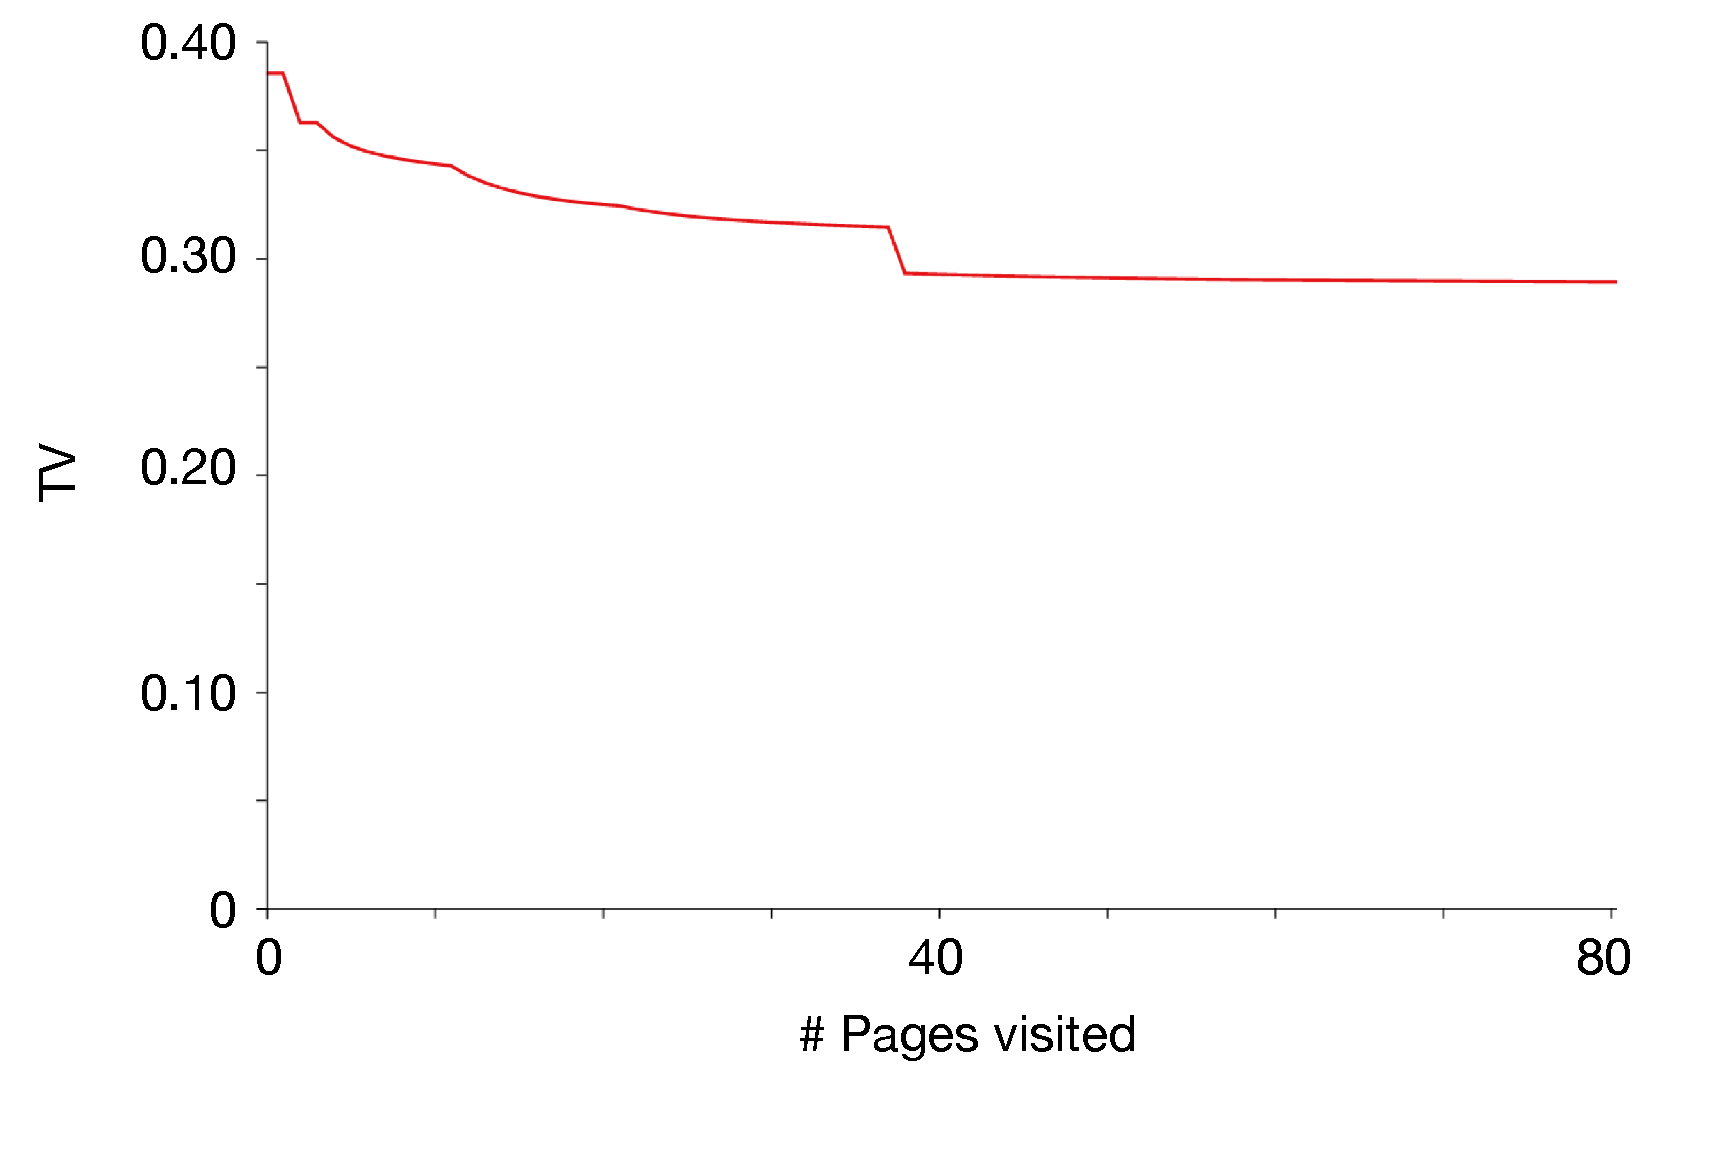
\includegraphics{figures/facebook-tracking-page-norm-1.eps}}}%
\subfigure[]{
\resizebox*{7cm}{!}{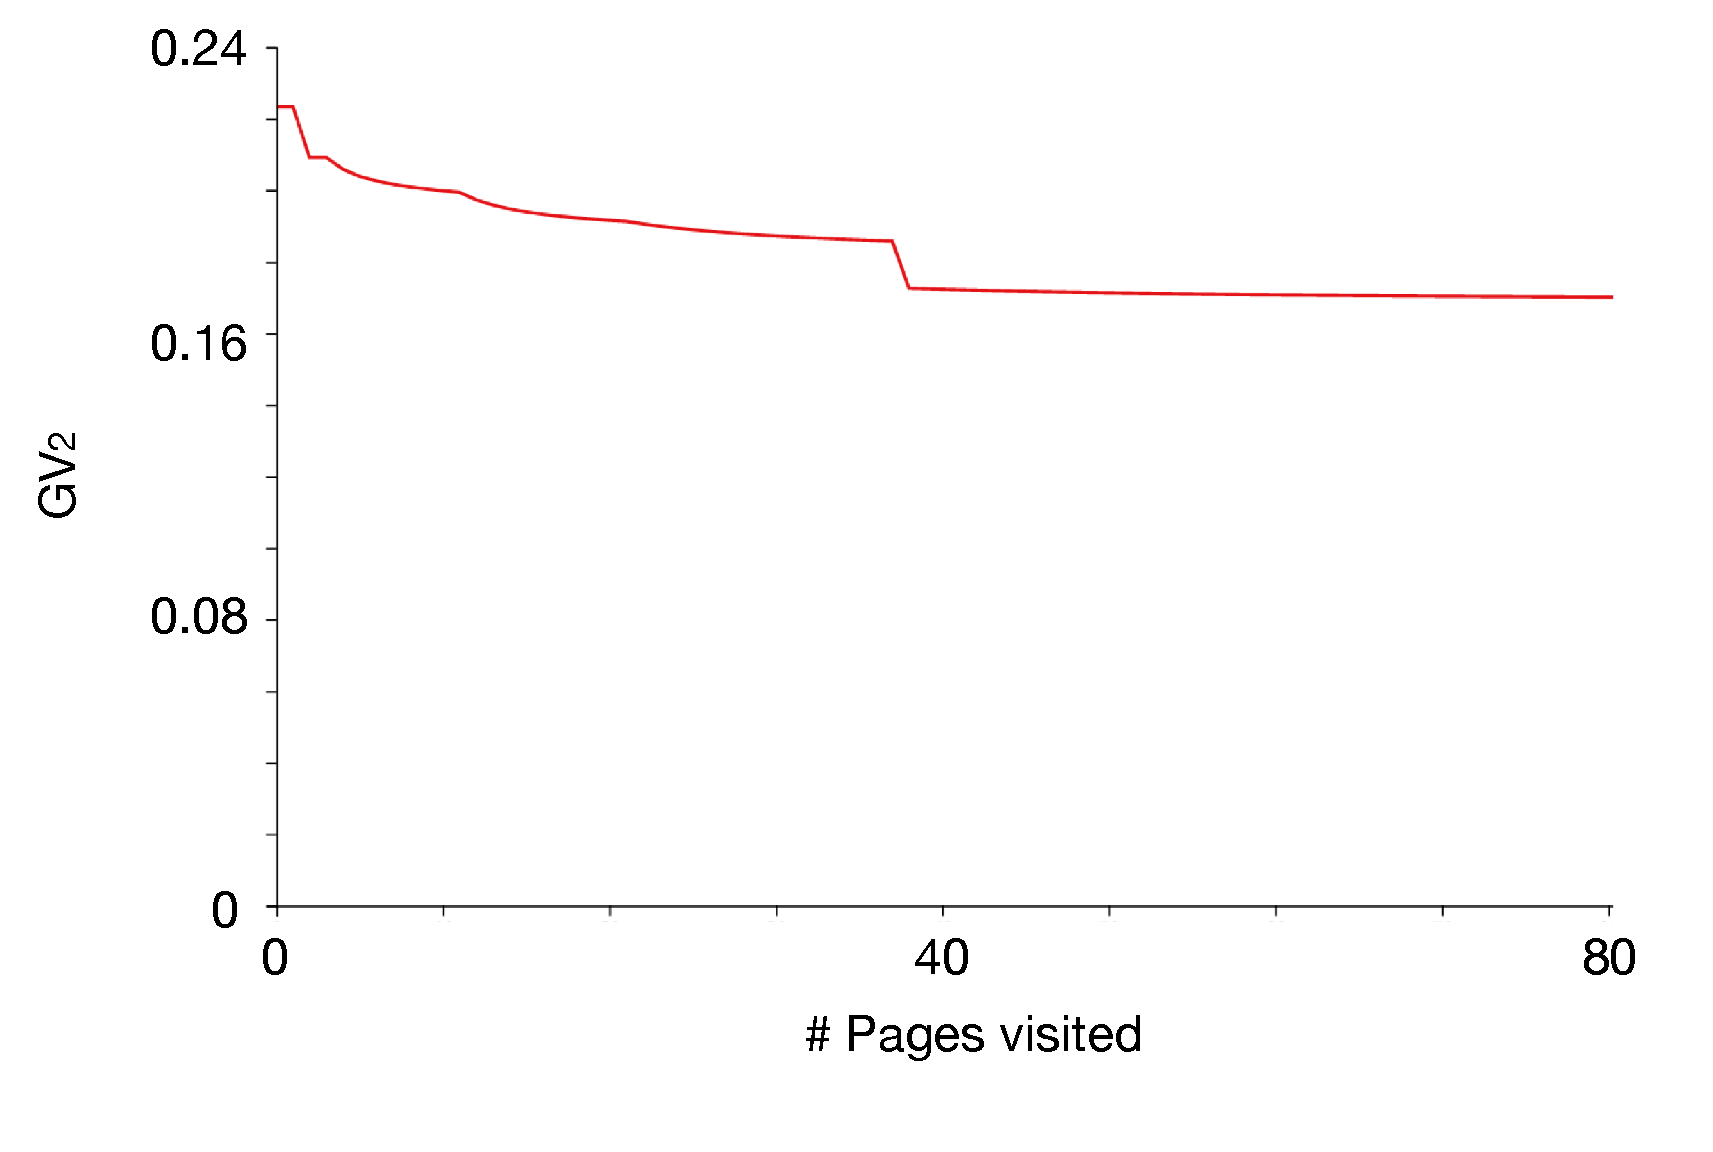
\includegraphics{figures/facebook-tracking-page-norm-2.eps}}}%


\subfigure[]{
\resizebox*{7cm}{!}{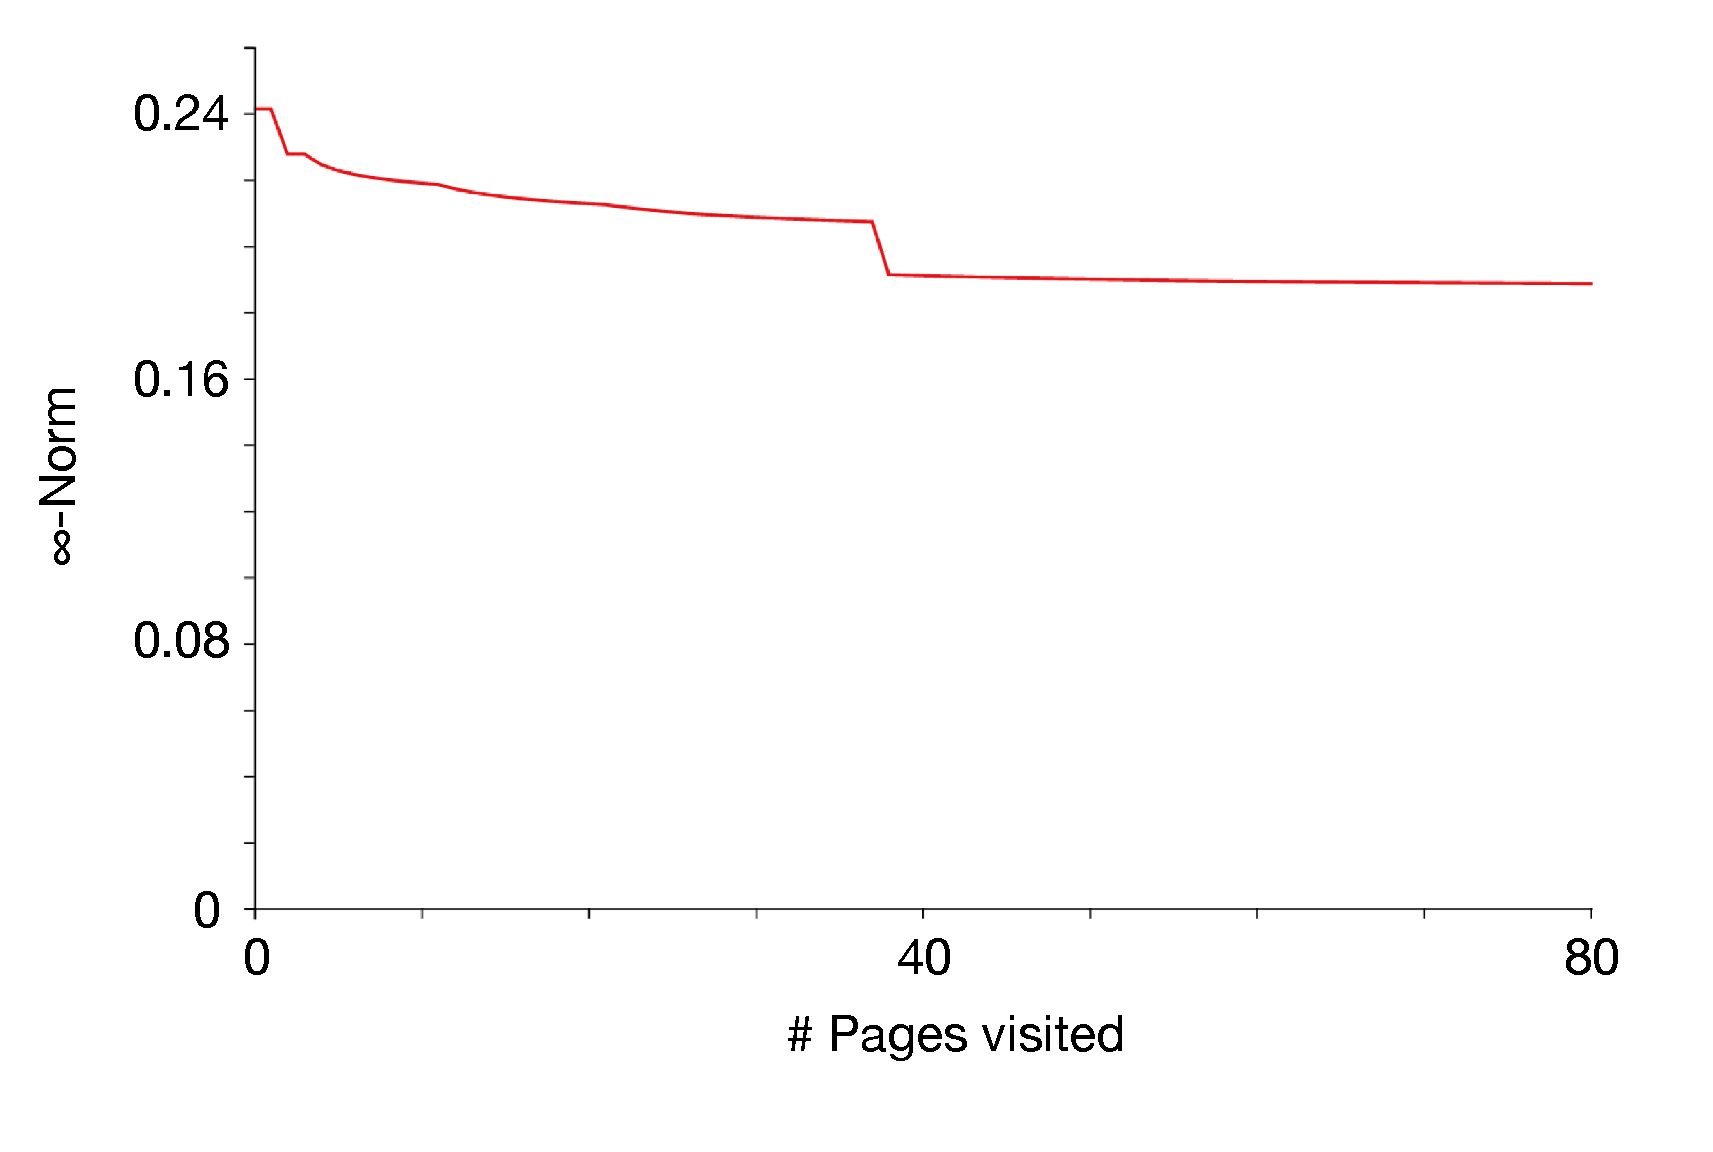
\includegraphics{figures/facebook-tracking-page-norm-inf.eps}}}%
\subfigure[]{
\resizebox*{7cm}{!}{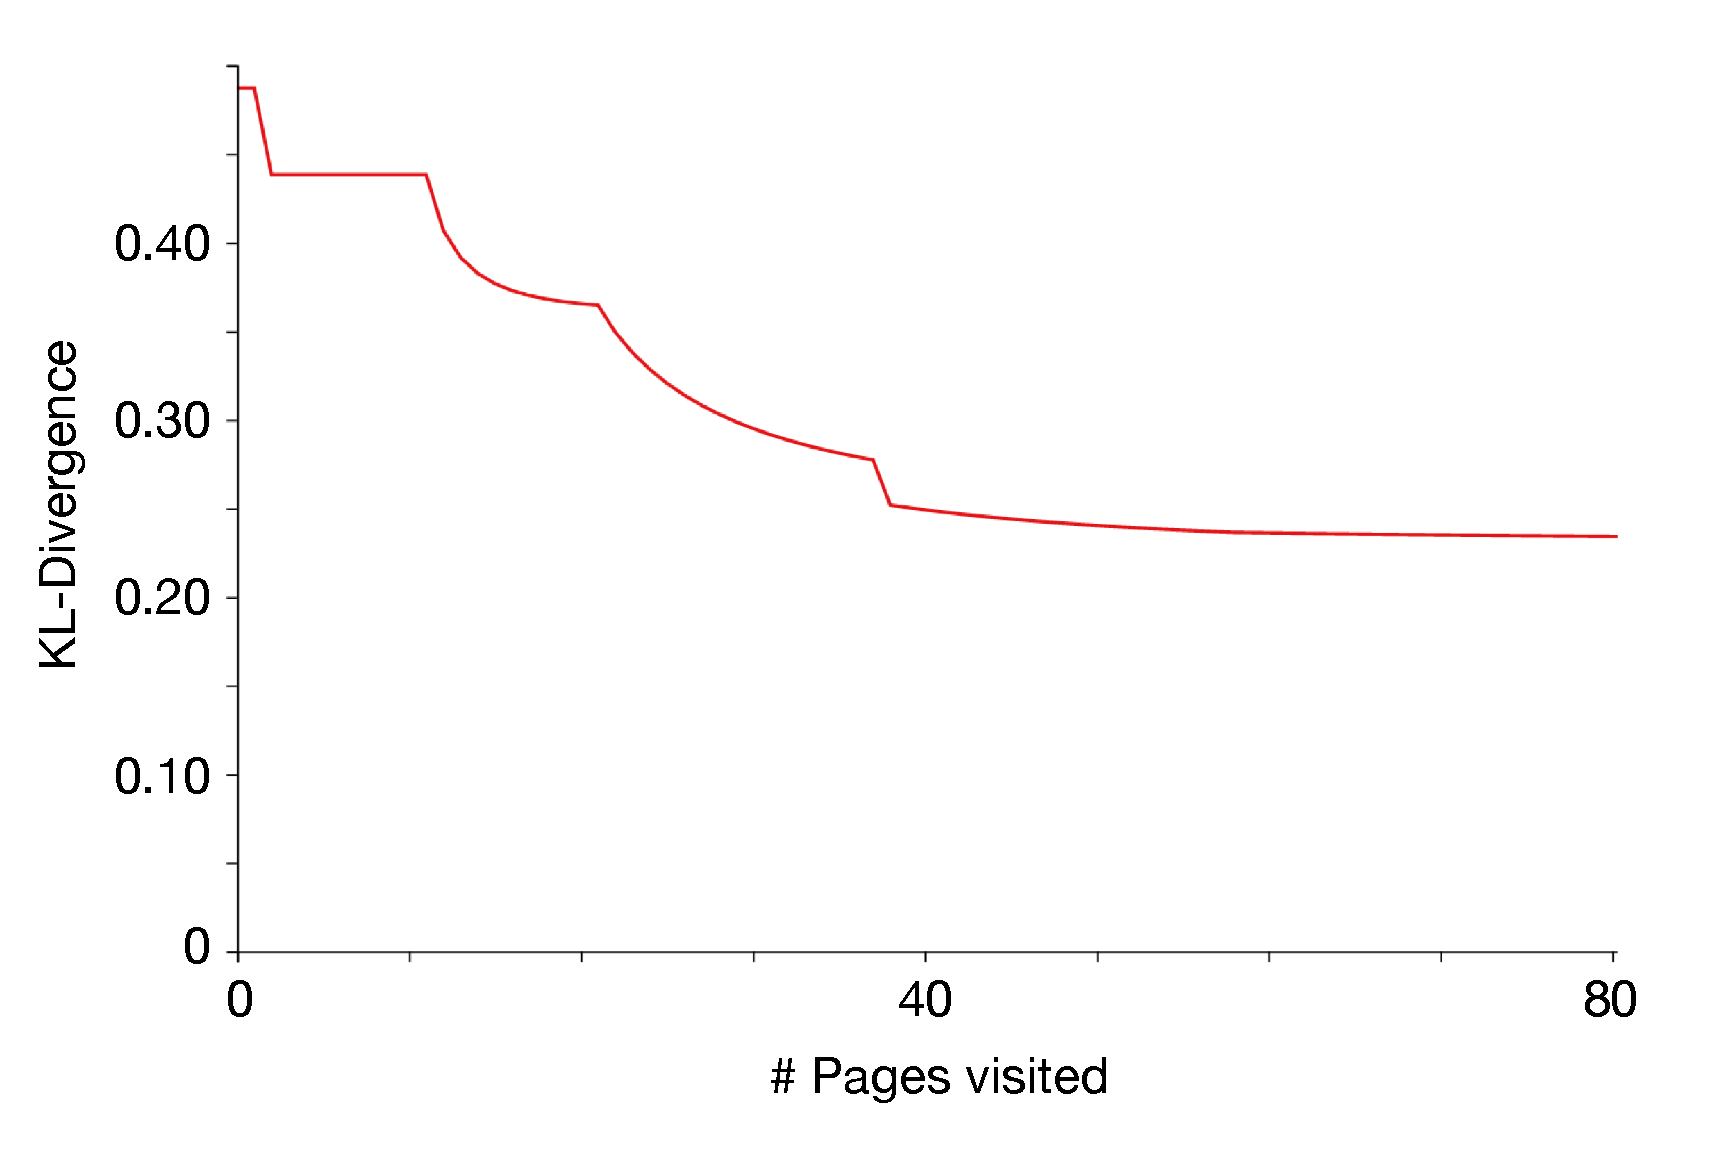
\includegraphics{figures/facebook-tracking-page-kl.eps}}}%
\caption{\label{average-facebook-pages-tracker} The figure show the relation between the profile captured by third-party requests to Facebook services and the actual user profile. Please recall that we calculated the user profile at the end of the series of 100 web pages visited and we calculated the metrics for 80 visits, giving a 80\% estimation.%
We therefore computed the \emph{TV}(a), the \emph{$GV_2$}(b), the \emph{$\infty$-norm}(c) and the \emph{KL-divergence}(d) for all pages and averaged among all users.}%
\end{center}
\end{figure}

\begin{figure}{10}
\begin{center}
\subfigure[]{
\resizebox*{7cm}{!}{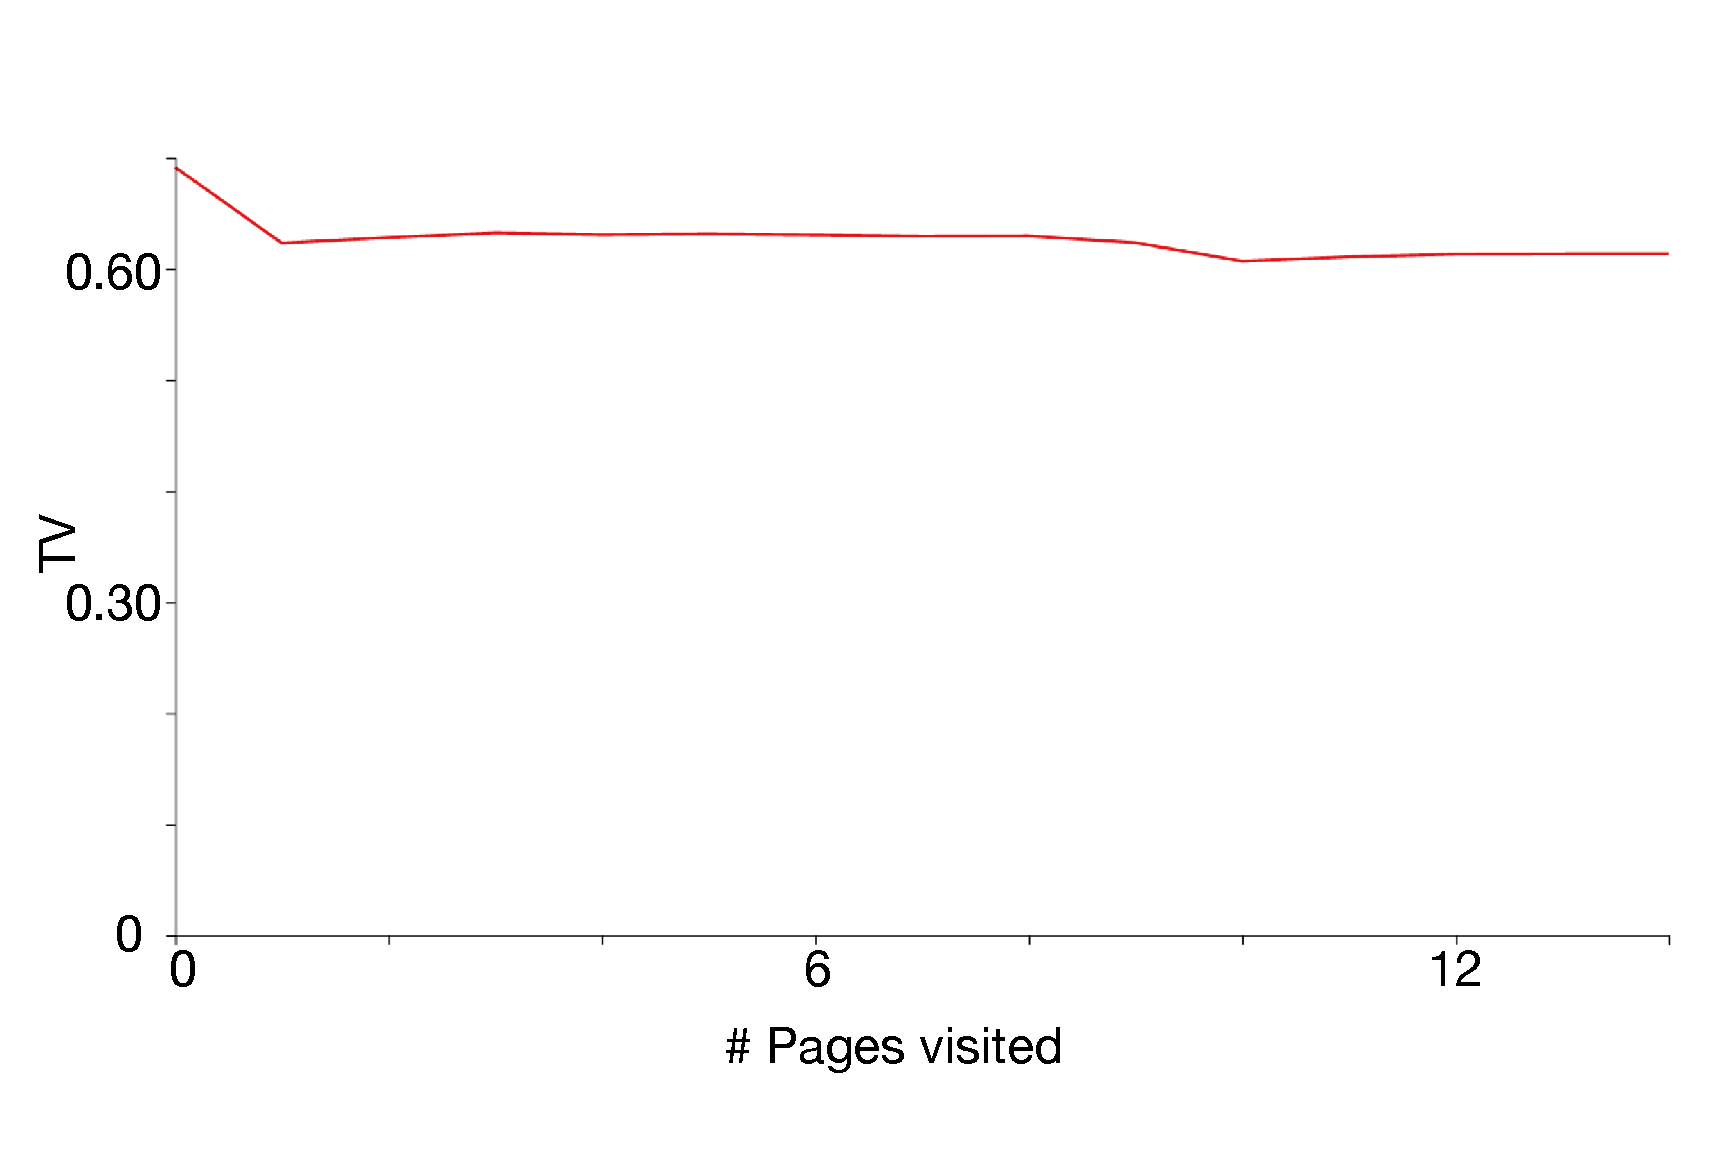
\includegraphics{figures/facebook-tracking-tags-norm-1.eps}}}%
\subfigure[]{
\resizebox*{7cm}{!}{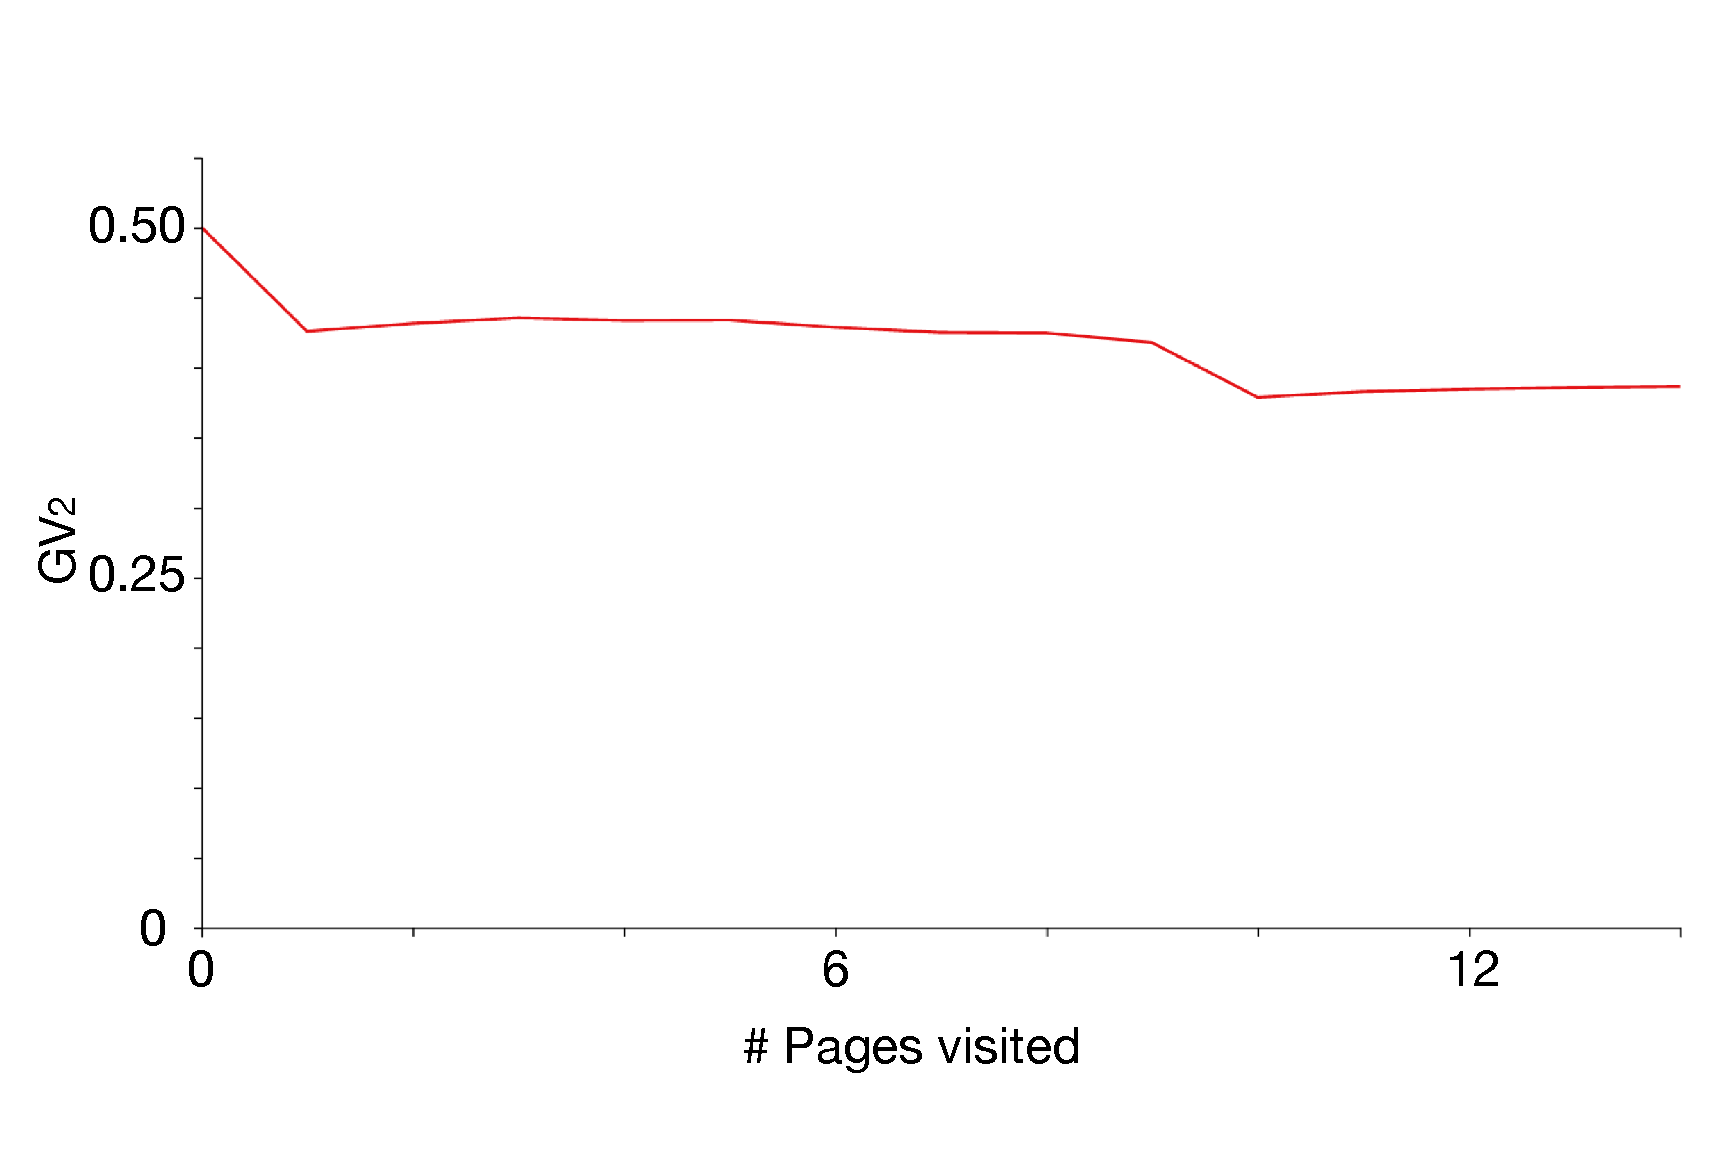
\includegraphics{figures/facebook-tracking-tags-norm-2.eps}}}%


\subfigure[]{
\resizebox*{7cm}{!}{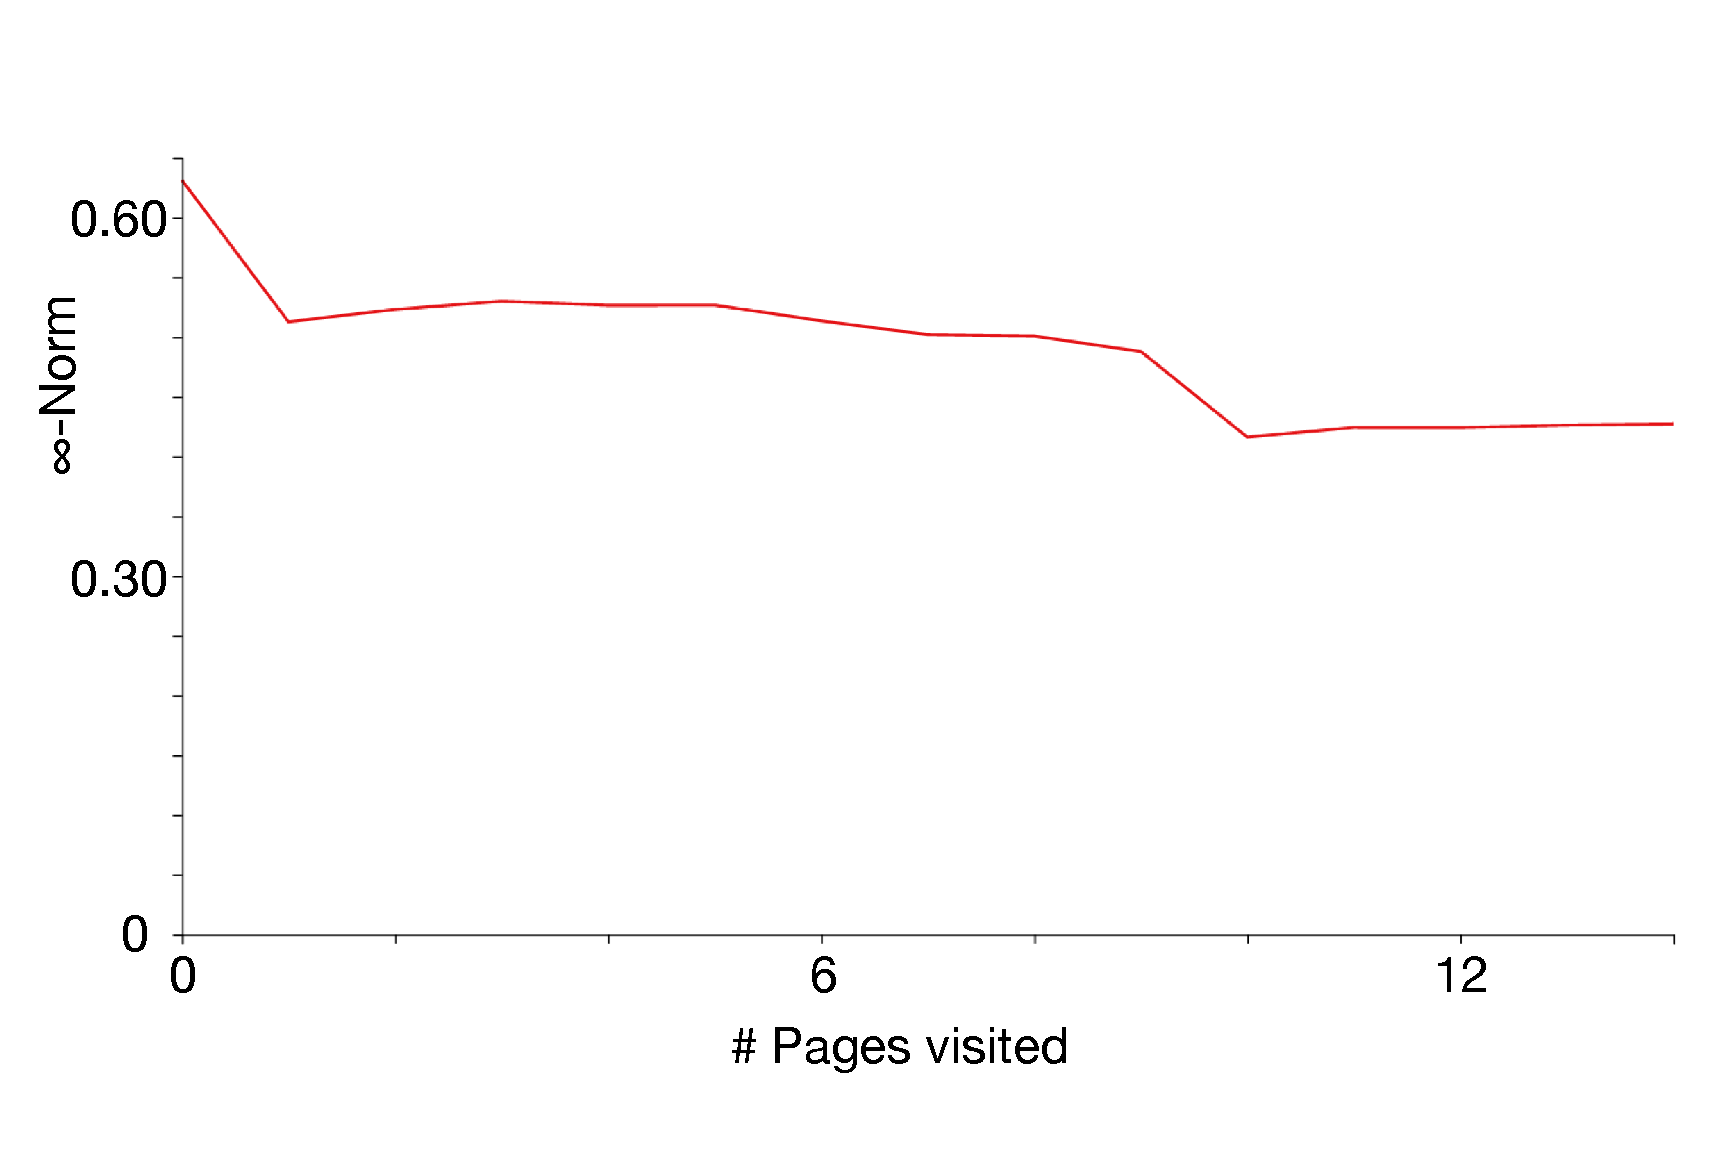
\includegraphics{figures/facebook-tracking-tags-norm-inf.eps}}}%
\subfigure[]{
\resizebox*{7cm}{!}{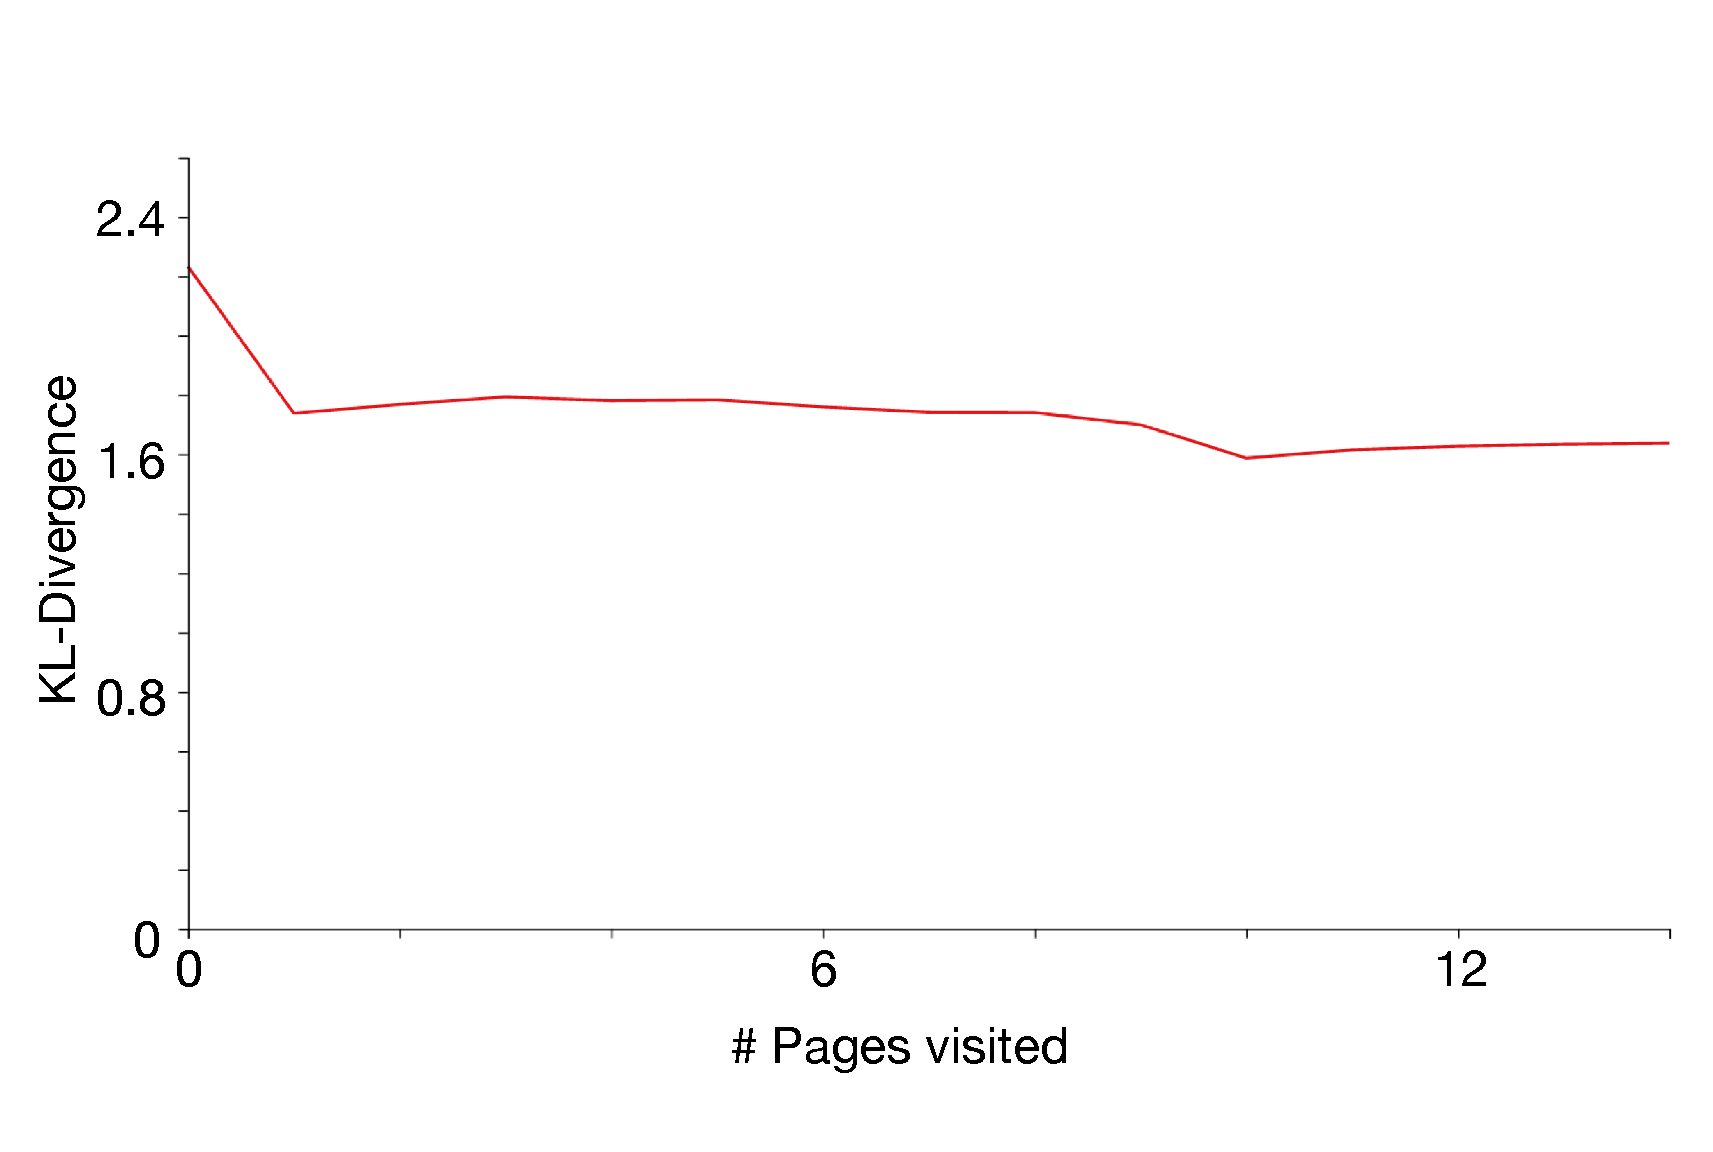
\includegraphics{figures/facebook-tracking-tags-kl.eps}}}%
\caption{\label{average-facebook-tags-tracker} The figure show the relation between the profile sent by third-party requests ($q_n$ with $n \in [1, N]$) to Facebook services and the actual user profile. Please recall that we calculated the user profile at the end of the series of 15 web pages visited. %
We therefore computed the \emph{TV}(a), the \emph{$GV_2$}(b), the \emph{$\infty$-norm}(c) and the \emph{KL-divergence}(d) for all http calls and averaged among all users.}%
\end{center}
\end{figure}

\section{Discussion}

We introduced a set of metrics to show how information is sent to third-party tracking services when users surf the web. Because we considered users that were not logged into any identity account, such as Twitter, Google+ or Facebook, we show how third-party service were still able to collect valuable information.
We computed the set of metrics for the partial user profile at each page visited. This shows how each page contribute to the actual user profile at the end of a series of websites visited. This means that an advertising network that is present on most of the pages visited possess a large amount of information regarding users and population of users. This information finally allows networks to predict fairly quickly user's preferences and behaviour.
We also computed a set of network analysis on our graph model of the user online footprint. We were able to identify known trackers and isolate communities of similar trackers. This aspect is particularly interesting for the development of Privacy Enhancing Technologies for the web. Up to now, anti-tracking technologies have been built to simply stop third-party requests, alternative strategies might instead consider to send bogus information to certain over-connected tracker domains to masquerade the user real profile. At the same time a measurement of the average degree of the neighbourhood of a certain third-party domain can be used to evaluate how \emph{dangerous} this can be considered for the user's privacy.
